% ============================================================
%  PROPOSAL SKRIPSI — UNIVERSITAS KRISTEN KRIDA WACANA (UKRIDA)
%  Fakultas Ekonomi dan Bisnis — Program Studi S1 Manajemen
%  Konsentrasi: Manajemen Keuangan
%  Judul: Pengaruh Hedonic Motivation, Desire for Completeness, dan
%         Speculative Motive terhadap Impulsive Buying Booster Pack
%         Kartu Pokemon TCG dengan Self-Control sebagai Variabel Moderasi
%  Format: Sesuai Buku Pedoman Penyusunan Tugas Akhir FEB UKRIDA 2023 (Model B)
%  Engine: XeLaTeX (Font: Times New Roman via fontspec)
% ============================================================

\documentclass[12pt,a4paper]{article}

% ---- ENCODING & FONT (Pedoman UKRIDA §3.2.b: Times New Roman 12pt) ----
\usepackage{fontspec}
\setmainfont{Times New Roman}

% ---- CAPTION & ISTILAH INDONESIA ----
\renewcommand{\tablename}{Tabel}
\renewcommand{\figurename}{Gambar}

% ---- HYPHENATION & EMERGENCE STRETCH ----
\hyphenation{he-te-ro-ske-das-ti-si-tas mul-ti-ko-li-ne-a-ri-tas au-to-ko-re-la-si li-te-ra-si pe-ran-cang-an gra-ti-fi-ca-tion kom-ple-ti-tas}
\setlength{\emergencystretch}{2.5em}

% ---- PAGE GEOMETRY (Pedoman UKRIDA §3.2.a: Kiri 4cm, Atas/Kanan/Bawah 3cm) ----
\usepackage[
  left=4cm,
  right=3cm,
  top=3cm,
  bottom=3cm,
  a4paper
]{geometry}

% ---- LINE SPACING (Pedoman UKRIDA §3.2.e: 1.5 Spasi) ----
\usepackage{setspace}
\onehalfspacing

% ---- PARAGRAPH INDENT (Pedoman UKRIDA §3.2.f: 5 ketukan ~ 1.25cm) ----
\usepackage{indentfirst}
\setlength{\parindent}{1.25cm}
\setlength{\parskip}{0pt}
\usepackage{enumitem}

% ---- TABEL & ARRAY (Desain Terbuka Standar Jurnal / Booktabs) ----
\usepackage{booktabs}
\usepackage{longtable}
\usepackage{tabularx}
\usepackage{array}
\usepackage{multirow}
\usepackage{makecell}
\renewcommand{\arraystretch}{1.35}

% ---- GAMBAR & CAPTION (Pedoman UKRIDA §3.2.g: Tabel judul di atas, Gambar di bawah) ----
\usepackage{graphicx}
\usepackage{float}
\usepackage{caption}
\captionsetup[table]{labelsep=period, justification=raggedright, singlelinecheck=false, position=top, font=small}
\captionsetup[figure]{labelsep=period, justification=centering, position=bottom, font=small}

% ---- MATEMATIKA ----
\usepackage{amsmath}
\usepackage{amssymb}

% ---- TIKZ (DIAGRAM KERANGKA KONSEPTUAL) ----
\usepackage{tikz}
\usetikzlibrary{shapes.geometric, arrows.meta, positioning, calc}

% ---- SECTION TITLE FORMATTING (Pedoman UKRIDA §3.2.c: BAB KAPITAL BOLD CENTER) ----
\usepackage{titlesec}
\titleformat{\section}[block]
  {\normalfont\fontsize{12}{14}\bfseries\centering\MakeUppercase}
  {}
  {0pt}
  {}
\titlespacing*{\section}{0pt}{18pt}{12pt}

\titleformat{\subsection}[block]
  {\normalfont\fontsize{12}{14}\bfseries}
  {\thesubsection.}
  {0.5em}
  {}
\titlespacing*{\subsection}{0pt}{12pt}{6pt}

\titleformat{\subsubsection}[block]
  {\normalfont\fontsize{12}{14}\bfseries}
  {\thesubsubsection.}
  {0.5em}
  {}
\titlespacing*{\subsubsection}{0pt}{10pt}{4pt}

% ---- HEADER & FOOTER (Pedoman UKRIDA §3.3.b & Jeddy: Accent Bar 4 di Kanan Bawah) ----
\usepackage{fancyhdr}
\pagestyle{fancy}
\fancyhf{}
\renewcommand{\headrulewidth}{0pt}
\renewcommand{\footrulewidth}{0pt}
\fancyfoot[R]{\footnotesize\textbf{Universitas Kristen Krida Wacana} $|$ \thepage}

% Halaman awal frontmatter: footer kanan bawah dengan penomoran romawi kecil
\fancypagestyle{frontmatter}{
  \fancyhf{}
  \renewcommand{\headrulewidth}{0pt}
  \renewcommand{\footrulewidth}{0pt}
  \fancyfoot[R]{\footnotesize\textbf{Universitas Kristen Krida Wacana} $|$ \thepage}
}

% Halaman plain / bab baru: footer kanan bawah konsisten
\fancypagestyle{plain}{
  \fancyhf{}
  \renewcommand{\headrulewidth}{0pt}
  \renewcommand{\footrulewidth}{0pt}
  \fancyfoot[R]{\footnotesize\textbf{Universitas Kristen Krida Wacana} $|$ \thepage}
}

% ---- DAFTAR ISI / TABEL / GAMBAR (tocloft) ----
\usepackage[titles]{tocloft}
\renewcommand{\cfttoctitlefont}{\hfill\large\bfseries}
\renewcommand{\cftaftertoctitle}{\hfill}
\renewcommand{\cftlottitlefont}{\hfill\large\bfseries}
\renewcommand{\cftafterlottitle}{\hfill}
\renewcommand{\cftloftitlefont}{\hfill\large\bfseries}
\renewcommand{\cftafterloftitle}{\hfill}

% Awalan Tabel dan Gambar di daftar
\renewcommand{\cfttabpresnum}{Tabel }
\renewcommand{\cfttabaftersnum}{.}
\setlength{\cfttabnumwidth}{2.3cm}
\renewcommand{\cftfigpresnum}{Gambar }
\renewcommand{\cftfigaftersnum}{.}
\setlength{\cftfignumwidth}{2.5cm}

% ---- BIBLIOGRAPHY (APA Style via natbib + apalike) ----
\usepackage{natbib}
\bibliographystyle{apalike}
\bibpunct{(}{)}{;}{a}{,}{,}

% ---- HYPERREF (Tautan Interaktif Digital, Teks Hitam Formal Sesuai Pedoman §3.2.i) ----
\usepackage[
  colorlinks=true,
  linkcolor=black,
  citecolor=black,
  urlcolor=black,
  bookmarks=true,
  bookmarksnumbered=true,
  pdfpagemode=UseOutlines
]{hyperref}

% ---- PENOMORAN OTOMATIS BERDASARKAN BAB ----
\numberwithin{equation}{section}
\numberwithin{table}{section}
\numberwithin{figure}{section}

% ---- METADATA MAHASISWA & PEMBIMBING ----
\newcommand{\ukrida}{Universitas Kristen Krida Wacana}
\newcommand{\feb}{Fakultas Ekonomi dan Bisnis}
\newcommand{\prodi}{Program Studi S1 Manajemen}
\newcommand{\konsentrasi}{Manajemen Keuangan}
\newcommand{\namamahasiswa}{Arthur Reezan}
\newcommand{\nim}{312023002}
\newcommand{\dosbim}{Dr. Fredella Colline, S.E., M.M., CFP\textsuperscript{\textregistered}, PFM, CHCP-A}
\newcommand{\nidn}{[NIDN\_DOSEN]}
\newcommand{\ketprodi}{Rita Amelinda, S.E., M.M.}
\newcommand{\judulskripsi}{PENGARUH \emph{HEDONIC MOTIVATION}, \emph{DESIRE FOR COMPLETENESS}, DAN \emph{SPECULATIVE MOTIVE} TERHADAP \emph{IMPULSIVE BUYING} \emph{BOOSTER PACK} KARTU POK\'EMON TCG DENGAN \emph{SELF-CONTROL} SEBAGAI VARIABEL MODERASI}

% ============================================================
%  DOKUMEN UTAMA
% ============================================================
\begin{document}

% ============================================================
%  BAGIAN AWAL — Penomoran Romawi Kecil
% ============================================================
\pagenumbering{roman}
\pagestyle{frontmatter}

% ------------------------------------------------------------
%  1. HALAMAN JUDUL LUAR / SAMPUL (hal. i)
% ------------------------------------------------------------
\thispagestyle{empty}
\begin{titlepage}
  \begin{center}
    \vspace*{0.2cm}
    
\includegraphics[width=3.2cm]{images/ukrida_pentagram.pdf}\\[0.8cm]

    {\large\bfseries PROPOSAL SKRIPSI}\\[1.2cm]

    {\large\bfseries
      PENGARUH \emph{HEDONIC MOTIVATION},\\
      \emph{DESIRE FOR COMPLETENESS}, DAN\\
      \emph{SPECULATIVE MOTIVE}\\
      TERHADAP \emph{IMPULSIVE BUYING} \emph{BOOSTER PACK}\\
      KARTU POK\'EMON TCG DENGAN \emph{SELF-CONTROL}\\
      SEBAGAI VARIABEL MODERASI
    }\\[1.2cm]

    {\normalsize Diajukan Kepada \prodi}\\[0.2cm]
    {\normalsize Untuk Menyusun Skripsi Sarjana Manajemen (S.M.)}\\[1.2cm]

    {\normalsize Diajukan Oleh:}\\[0.4cm]
    {\large\bfseries \namamahasiswa}\\[0.2cm]
    {\large\bfseries (\nim)}\\[1.8cm]

    \vfill

    {\large\bfseries \feb}\\[0.3cm]
    {\large\bfseries \ukrida}\\[0.3cm]
    {\large\bfseries JAKARTA 2026}
  \end{center}
\end{titlepage}

\addtocounter{page}{1}

% (Modular 23 Sep 2026: Pernyataan Keaslian hidup mandiri di
%  01_Lembar_Persetujuan_Proposal/01_Pernyataan_Keaslian.docx)

% (Modular 23 Sep 2026: Persetujuan hidup mandiri di
%  01_Lembar_Persetujuan_Proposal/02_Halaman_Persetujuan.docx)

% (Modular 23 Sep 2026: Pengesahan hidup mandiri di
%  01_Lembar_Persetujuan_Proposal/03_Halaman_Pengesahan_Penguji.docx)

% (Modular 23 Sep 2026: Kata Pengantar hidup mandiri di
%  01_Lembar_Persetujuan_Proposal/04_Kata_Pengantar.docx)

% (Modular 23 Sep 2026: ABSTRAK hidup mandiri di
%  01_Lembar_Persetujuan_Proposal/05_Abstrak_Indonesia.docx —
%  isi: tujuan, metode cross-sectional Likert 5 poin N=120-150, novelty S-O-R +
%  kolektor + regulasi diri + behavioral finance, kata kunci 8 frasa)

% (Modular 23 Sep 2026: ABSTRACT hidup mandiri di
%  01_Lembar_Persetujuan_Proposal/06_Abstract_English.docx)

% ------------------------------------------------------------
%  2. DAFTAR ISI
% ------------------------------------------------------------
\newpage
\thispagestyle{frontmatter}
\renewcommand{\contentsname}{DAFTAR ISI}
\tableofcontents
\addtocontents{toc}{\protect\thispagestyle{frontmatter}}

% ------------------------------------------------------------
%  3. DAFTAR TABEL
% ------------------------------------------------------------
\newpage
\thispagestyle{frontmatter}
\renewcommand{\listtablename}{DAFTAR TABEL}
\listoftables
\addcontentsline{toc}{section}{DAFTAR TABEL}
\addtocontents{lot}{\protect\thispagestyle{frontmatter}}

% ------------------------------------------------------------
%  4. DAFTAR GAMBAR
% ------------------------------------------------------------
\newpage
\thispagestyle{frontmatter}
\renewcommand{\listfigurename}{DAFTAR GAMBAR}
\listoffigures
\addcontentsline{toc}{section}{DAFTAR GAMBAR}
\addtocontents{lof}{\protect\thispagestyle{frontmatter}}

% ============================================================
%  BAGIAN INTI / UTAMA — Penomoran Angka Arab (Mulai hal. 1)
% ============================================================
\newpage
\pagenumbering{arabic}
\pagestyle{fancy}

% ============================================================
%  BAB 1: PENDAHULUAN
% ============================================================
\setcounter{section}{0}
\section*{BAB 1\\[0.3cm]PENDAHULUAN}
\addcontentsline{toc}{section}{\texorpdfstring{BAB 1\quad PENDAHULUAN}{BAB 1 PENDAHULUAN}}
\setcounter{section}{1}
\setcounter{subsection}{0}
\setcounter{table}{0}
\setcounter{figure}{0}
\setcounter{equation}{0}

\subsection{Latar Belakang Penelitian}

Waralaba media (\emph{media franchise}) Pok\'emon yang diciptakan oleh Satoshi Tajiri bersama Game Freak dan diluncurkan oleh Nintendo pada tahun 1996 di Jepang telah berkembang menjadi fenomena budaya pop global paling berpengaruh di dunia. Berdasarkan data agregasi industri media internasional, Pok\'emon dinobatkan sebagai waralaba media dengan pendapatan tertinggi sepanjang masa (\emph{the highest-grossing media franchise in history}), dengan estimasi pendapatan kotor kumulatif melampaui US\$ 100,0 miliar \citep{statista2024pokemon}. Angka ini melampaui waralaba legendaris dunia lainnya seperti \emph{Hello Kitty}, \emph{Winnie the Pooh}, \emph{Mickey Mouse}, maupun \emph{Star Wars}. Keberhasilan ini ditopang ekosistem multimedia yang saling memperkuat: lini permainan video (dari RPG Generasi I di Game Boy hingga Generasi IX di Switch, serta \emph{Pok\'emon GO}, \emph{UNITE}, dan \emph{TCG Pocket}); lini animasi dan film (anime 25 tahun Satoshi dan Pikachu di 190 negara, \emph{The First Movie} (1998), \emph{Detective Pikachu} (2019), dan \emph{Horizons}); serta lini lisensi, gerai \emph{Pok\'emon Center}, dan turnamen tahunan \emph{World Championships}.

Berdasarkan data komparasi industri media global, dominasi ekonomi waralaba Pok\'emon disajikan pada Gambar 1.1.

\begin{figure}[htbp]
  \centering
  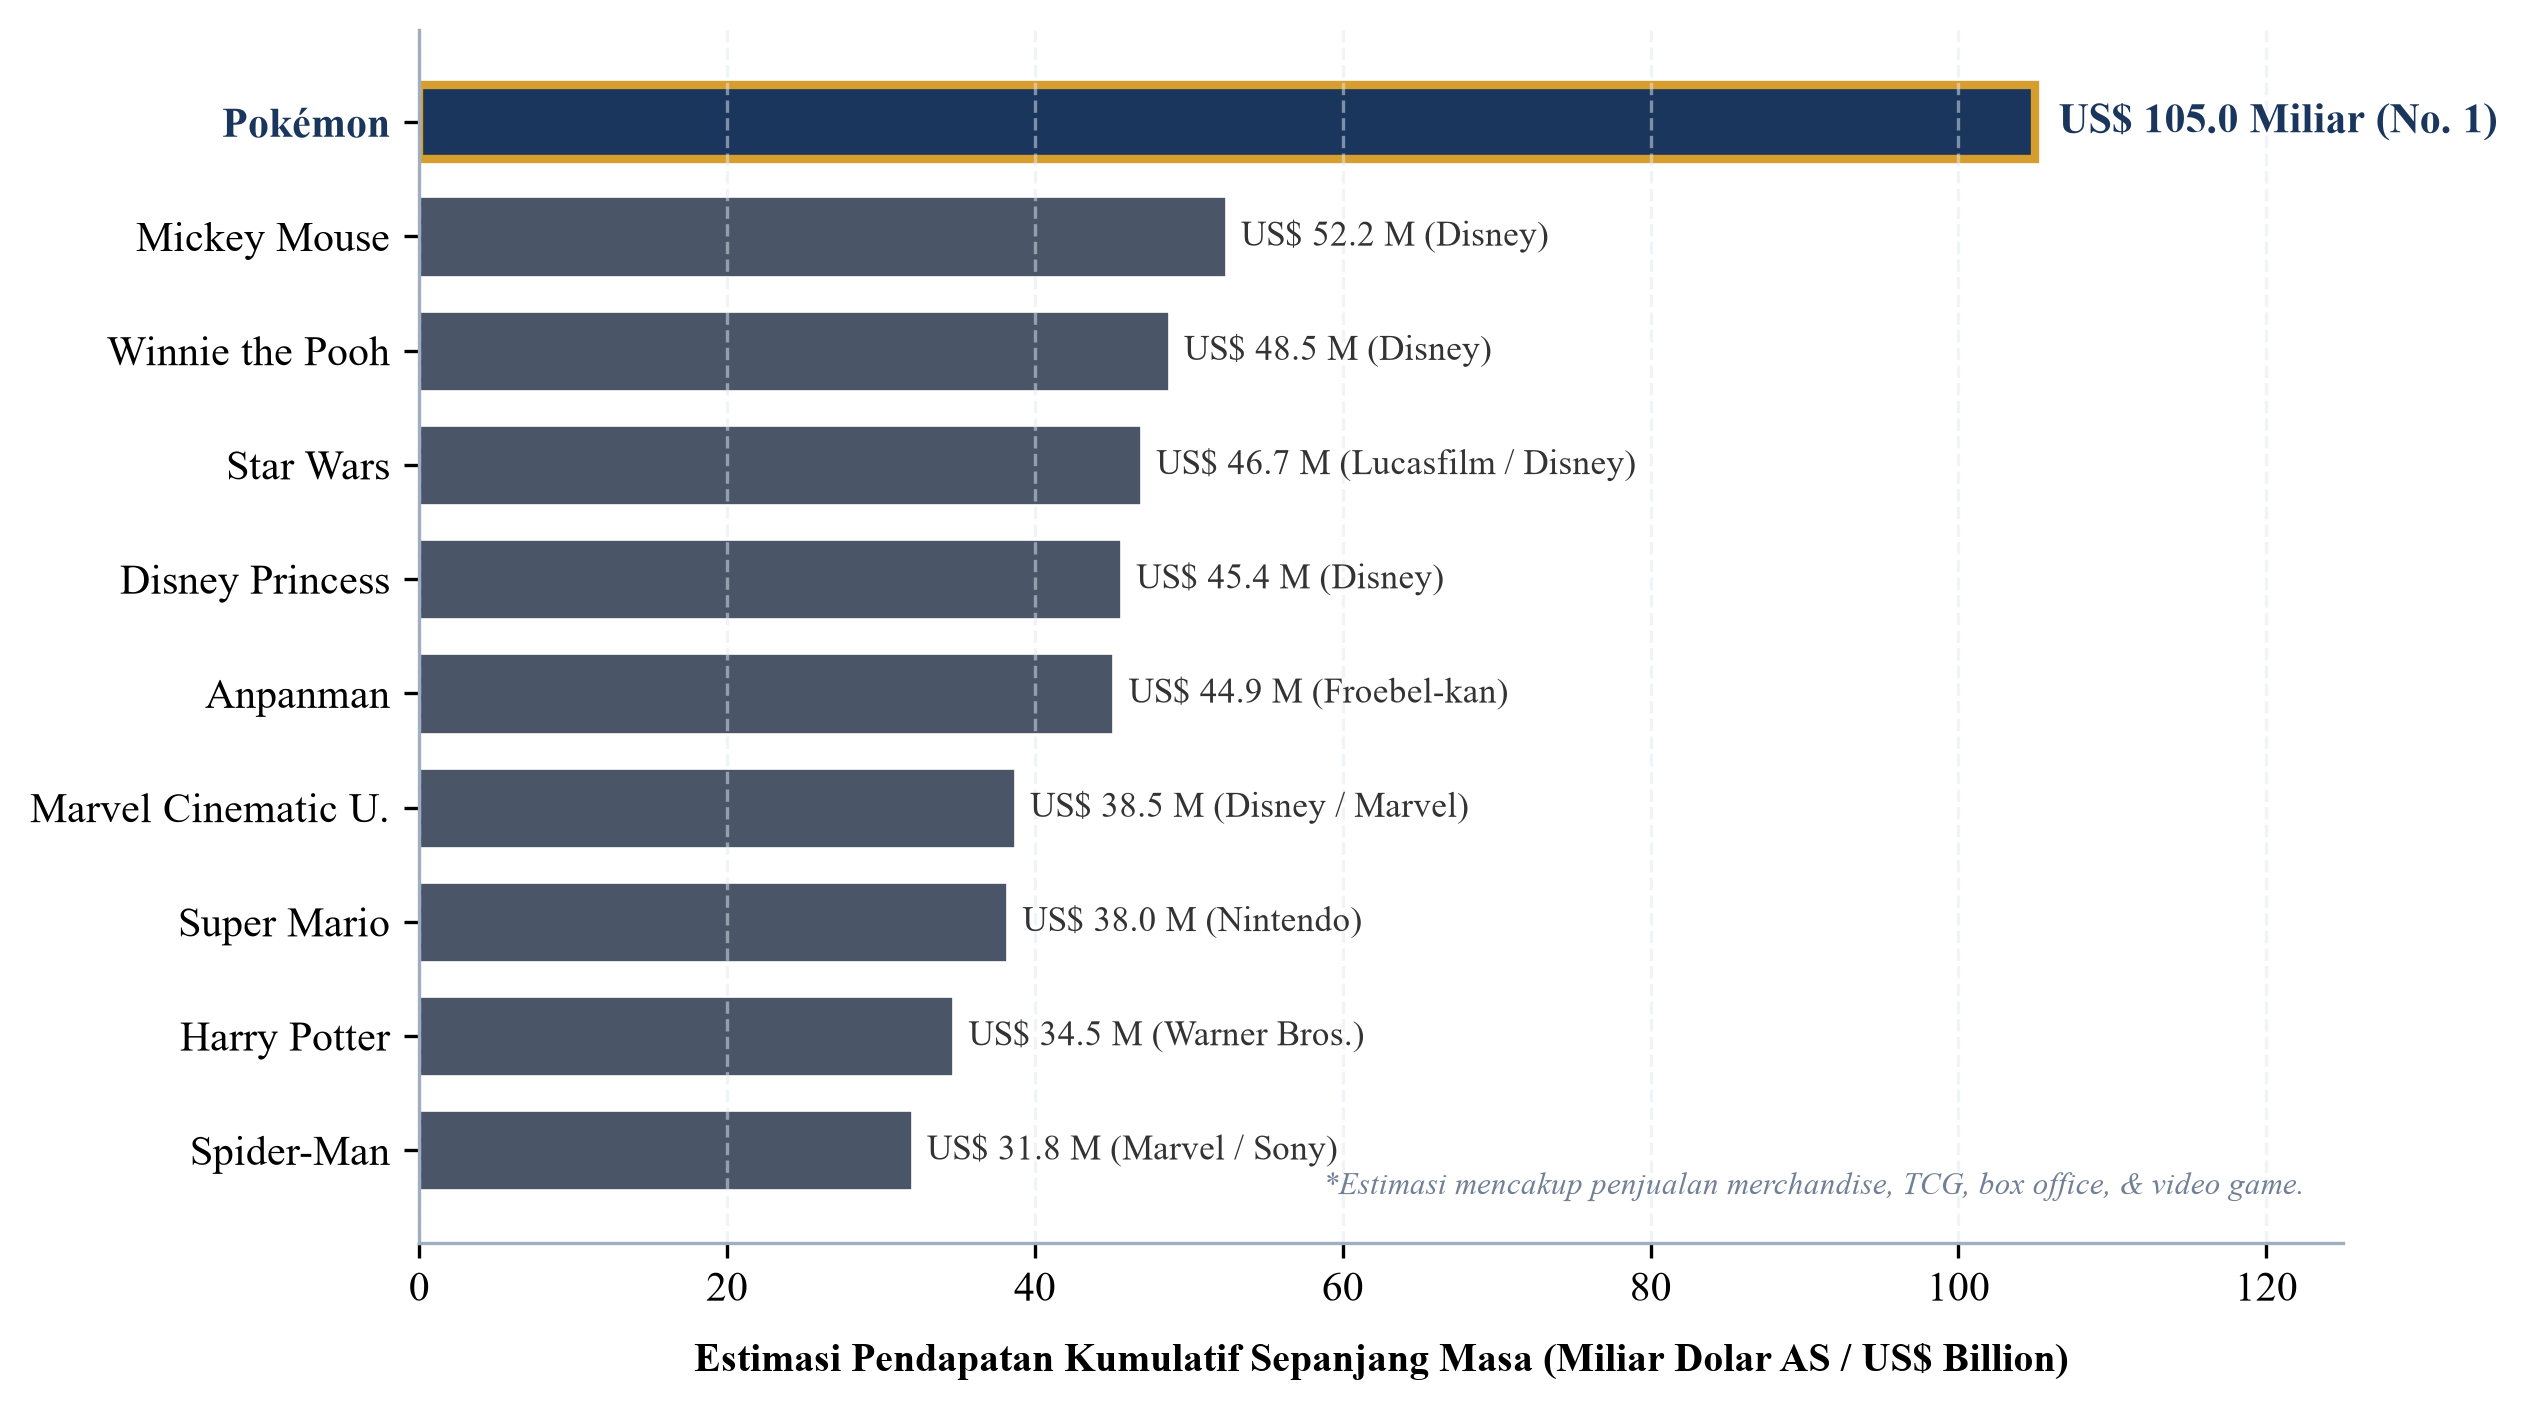
\includegraphics[width=0.80\textwidth]{images/gambar1_1_media_franchise_ranking.png}
  \caption{Peringkat 10 Waralaba Media Berpendapatan Tertinggi di Dunia Sepanjang Masa}
  \label{fig:media_franchise_ranking}
  \vspace{0.1cm}
  {\footnotesize \textit{Sumber: Statista Chart 24277 (terbit Februari 2021; diakses September 2026) dan Laporan Keuangan Tahunan Korporat}\par}
\end{figure}

Sebagaimana ditunjukkan pada Gambar 1.1, Pok\'emon menempati posisi puncak sebagai waralaba media nomor satu di dunia dengan total pendapatan melampaui US\$ 100,0 miliar \citep{statista2024pokemon}. Bukti empiris ini mengonfirmasi bahwa Pok\'emon bukan sekadar hiburan musiman anak-anak, melainkan entitas komersial raksasa dengan basis perputaran kapital lintas generasi yang sangat kokoh.

Di antara seluruh pilar ekosistem multimedia tersebut, \textbf{permainan kartu fisik atau \emph{Pok\'emon Trading Card Game} (Pok\'emon TCG)} memegang peranan yang paling sentral dan memiliki salah satu perputaran ekonomi koleksi fisik (\emph{physical collectibles}) terbesar di dunia. Hingga tahun 2024, The Pok\'emon Company mencatat bahwa produksi kumulatif kartu Pok\'emon fisik telah menembus lebih dari 64,8 miliar lembar kartu yang didistribusikan ke lebih dari 93 wilayah dan diterjemahkan ke dalam berbagai bahasa dunia \citep{pokemoncompany2024}. Kartu Pok\'emon bukan lagi sekadar alat permainan meja (\emph{tabletop game}) anak-anak, melainkan telah bertransformasi menjadi \textbf{instrumen aset alternatif koleksi (\emph{alternative collectibles asset})} bernilai ekonomi tinggi yang diperdagangkan secara aktif oleh kalangan dewasa muda, investor hobi, dan balai lelang global. Akselerasi pertumbuhan produksi kartu Pok\'emon TCG secara global diilustrasikan pada Gambar 1.2.

\begin{figure}[htbp]
  \centering
  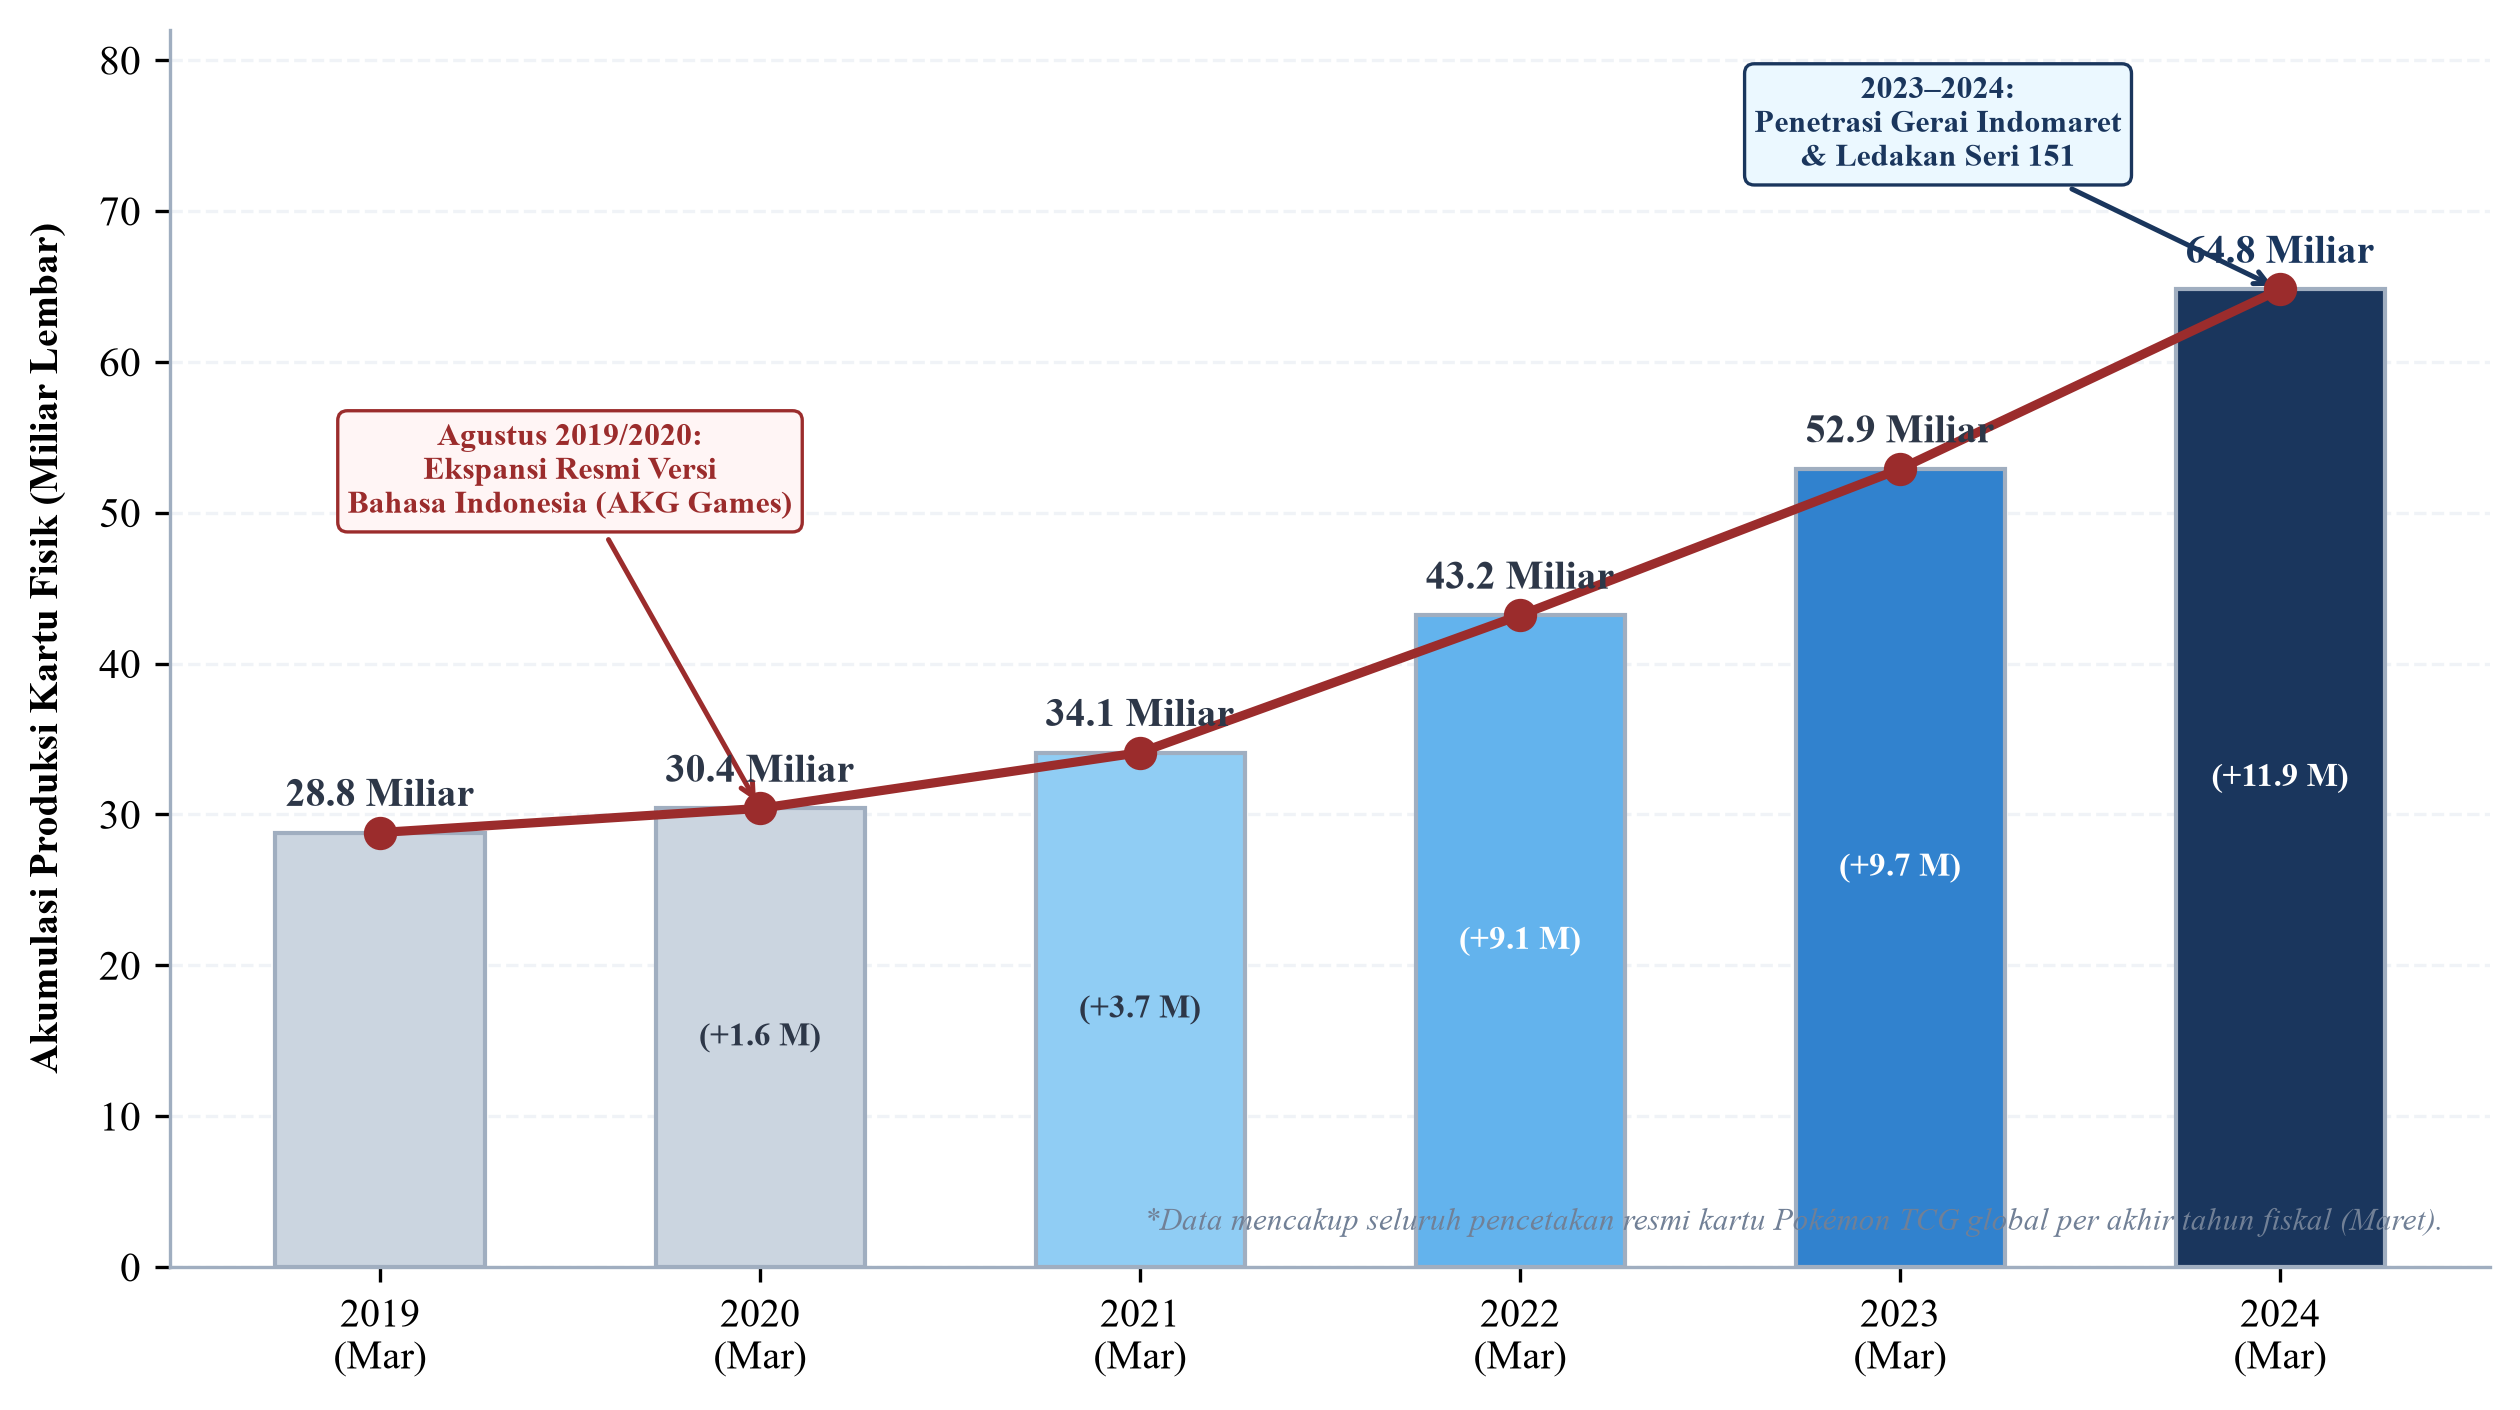
\includegraphics[width=0.80\textwidth]{images/gambar1_2_pokemon_tcg_production_growth.png}
  \caption{Pertumbuhan Kumulatif Produksi Kartu Pok\'emon TCG Global Tahun 2019--2024}
  \label{fig:pokemon_card_growth}
  \vspace{0.1cm}
  {\footnotesize \textit{Sumber: The Pok\'emon Company Corporate Business Data (2024)}\par}
\end{figure}

Berdasarkan Gambar 1.2, terlihat jelas terjadinya lonjakan produksi kartu fisik yang sangat tajam dalam lima tahun terakhir. Pada Maret 2019, total produksi kumulatif global tercatat sebesar 28,8 miliar lembar kartu. Namun, pasca dimulainya ekspansi pencetakan kartu versi resmi bahasa lokal, termasuk peluncuran resmi kartu berbahasa Indonesia pada Agustus 2019 serta meledaknya tren hobi koleksi fisik selama masa pandemi, akumulasi produksi meroket sebesar 125\% hingga menembus 64,8 miliar lembar kartu pada Maret 2024 \citep{pokemoncompany2024}. Pencetakan lebih dari 11,9 miliar lembar kartu hanya dalam kurun waktu satu tahun fiskal (2023--2024) mengindikasikan tingginya permintaan pasar dan mengonfirmasi terjadinya gelombang antusiasme belanja yang masif di kalangan konsumen.

Di Indonesia, kartu resmi Pok\'emon TCG berbahasa Indonesia hadir sejak 2019 melalui AKG Games dan didistribusikan agresif di ribuan gerai ritel modern (Indomaret, Alfamart, Gramedia, Toys Kingdom), tidak hanya di toko hobi khusus. Penempatan di etalase kasir mengubah hobi ceruk menjadi konsumsi populer nasional dan menciptakan pasar sekunder yang likuid. Minat masyarakat, khususnya mahasiswa dan Generasi Z, didorong oleh konvergensi fungsi rekreasi, prestise sosial, hobi koleksi kartu langka, dan motif spekulasi finansial.

Dinamika pasar Pok\'emon TCG fisik di Indonesia memunculkan fenomena perilaku konsumsi yang sangat unik sekaligus problematis. Produk kartu fisik dijual dalam format kemasan acak tertutup (\emph{blind pack} atau \emph{booster pack}) dengan harga eceran resmi yang sangat terjangkau, berkisar antara Rp20.000 hingga Rp30.000 per bungkus (berisi 5 lembar kartu acak). Namun, di dalam bungkus tersebut tersimpan peluang probabilitas untuk menarik kartu dengan tingkat kelangkaan tinggi (\emph{Special Illustration Rare / SAR}, kartu \emph{Super Rare / SR}, atau \emph{Ultra Rare / UR}). Di pasar sekunder daring (Tokopedia, Shopee, grup lelang Facebook, dan komunitas media sosial), kartu-kartu berkarakter favorit (seperti Charizard, Pikachu, atau kartu pelatih wanita/waifu populer) diperjualbelikan dengan harga fantastis mulai dari ratusan ribu hingga puluhan juta rupiah per lembar (lih.\ pantauan pasar sekunder \citep{pricecharting2024}).

Fenomena disparitas harga pasar sekunder ini diperkuat oleh keberadaan industri \textbf{sertifikasi penilaian kondisi fisik kartu (\emph{card grading})}. Lembaga \emph{grading} independen berstandar internasional terkemuka seperti \textbf{PSA (\emph{Professional Sports Authenticator})}, \textbf{BGS (\emph{Beckett Grading Services})}, dan \textbf{CGC Cards} memeriksa integritas fisik kartu secara mikroskopis berdasarkan empat kriteria utama: \emph{centering} (kesimetrisan cetak), \emph{surface} (kebersihan permukaan tanpa goresan), \emph{edges} (kerapian tepi), dan \emph{corners} (ketajaman sudut kartu). Kartu yang memenuhi kesempurnaan tertinggi akan disegel permanen dalam wadah akrilik kedap udara (\emph{tamper-evident slab}) dan diberi label skor kualitas 1 hingga 10 (\emph{PSA 10 Gem Mint} atau \emph{BGS 10 Pristine}). Kartu berpredikat \emph{Gem Mint 10} secara instan bertransformasi menjadi aset terstandardisasi yang likuid di bursa lelang global dengan harga jual yang terobservasi melonjak berkali-kali lipat dibandingkan kartu mentah (\emph{raw card}) \citep{pricecharting2024}. Kehadiran pasar \emph{grading} ini memicu gelombang spekulasi (\emph{grading arbitrage}), di mana konsumen tergiur membeli \emph{booster pack} murah dengan harapan menarik kartu berkondisi sempurna untuk digrade dan dijual kembali demi mendulang keuntungan modal (\emph{capital gain}).

Disparitas harga pasar sekunder yang ekstrem antara kartu mentah (\emph{ungraded}) dengan kartu berkondisi sempurna yang telah memperoleh sertifikasi \emph{PSA 10 Gem Mint} pada seri Pok\'emon populer disajikan pada Gambar 1.3.

\begin{figure}[htbp]
  \centering
  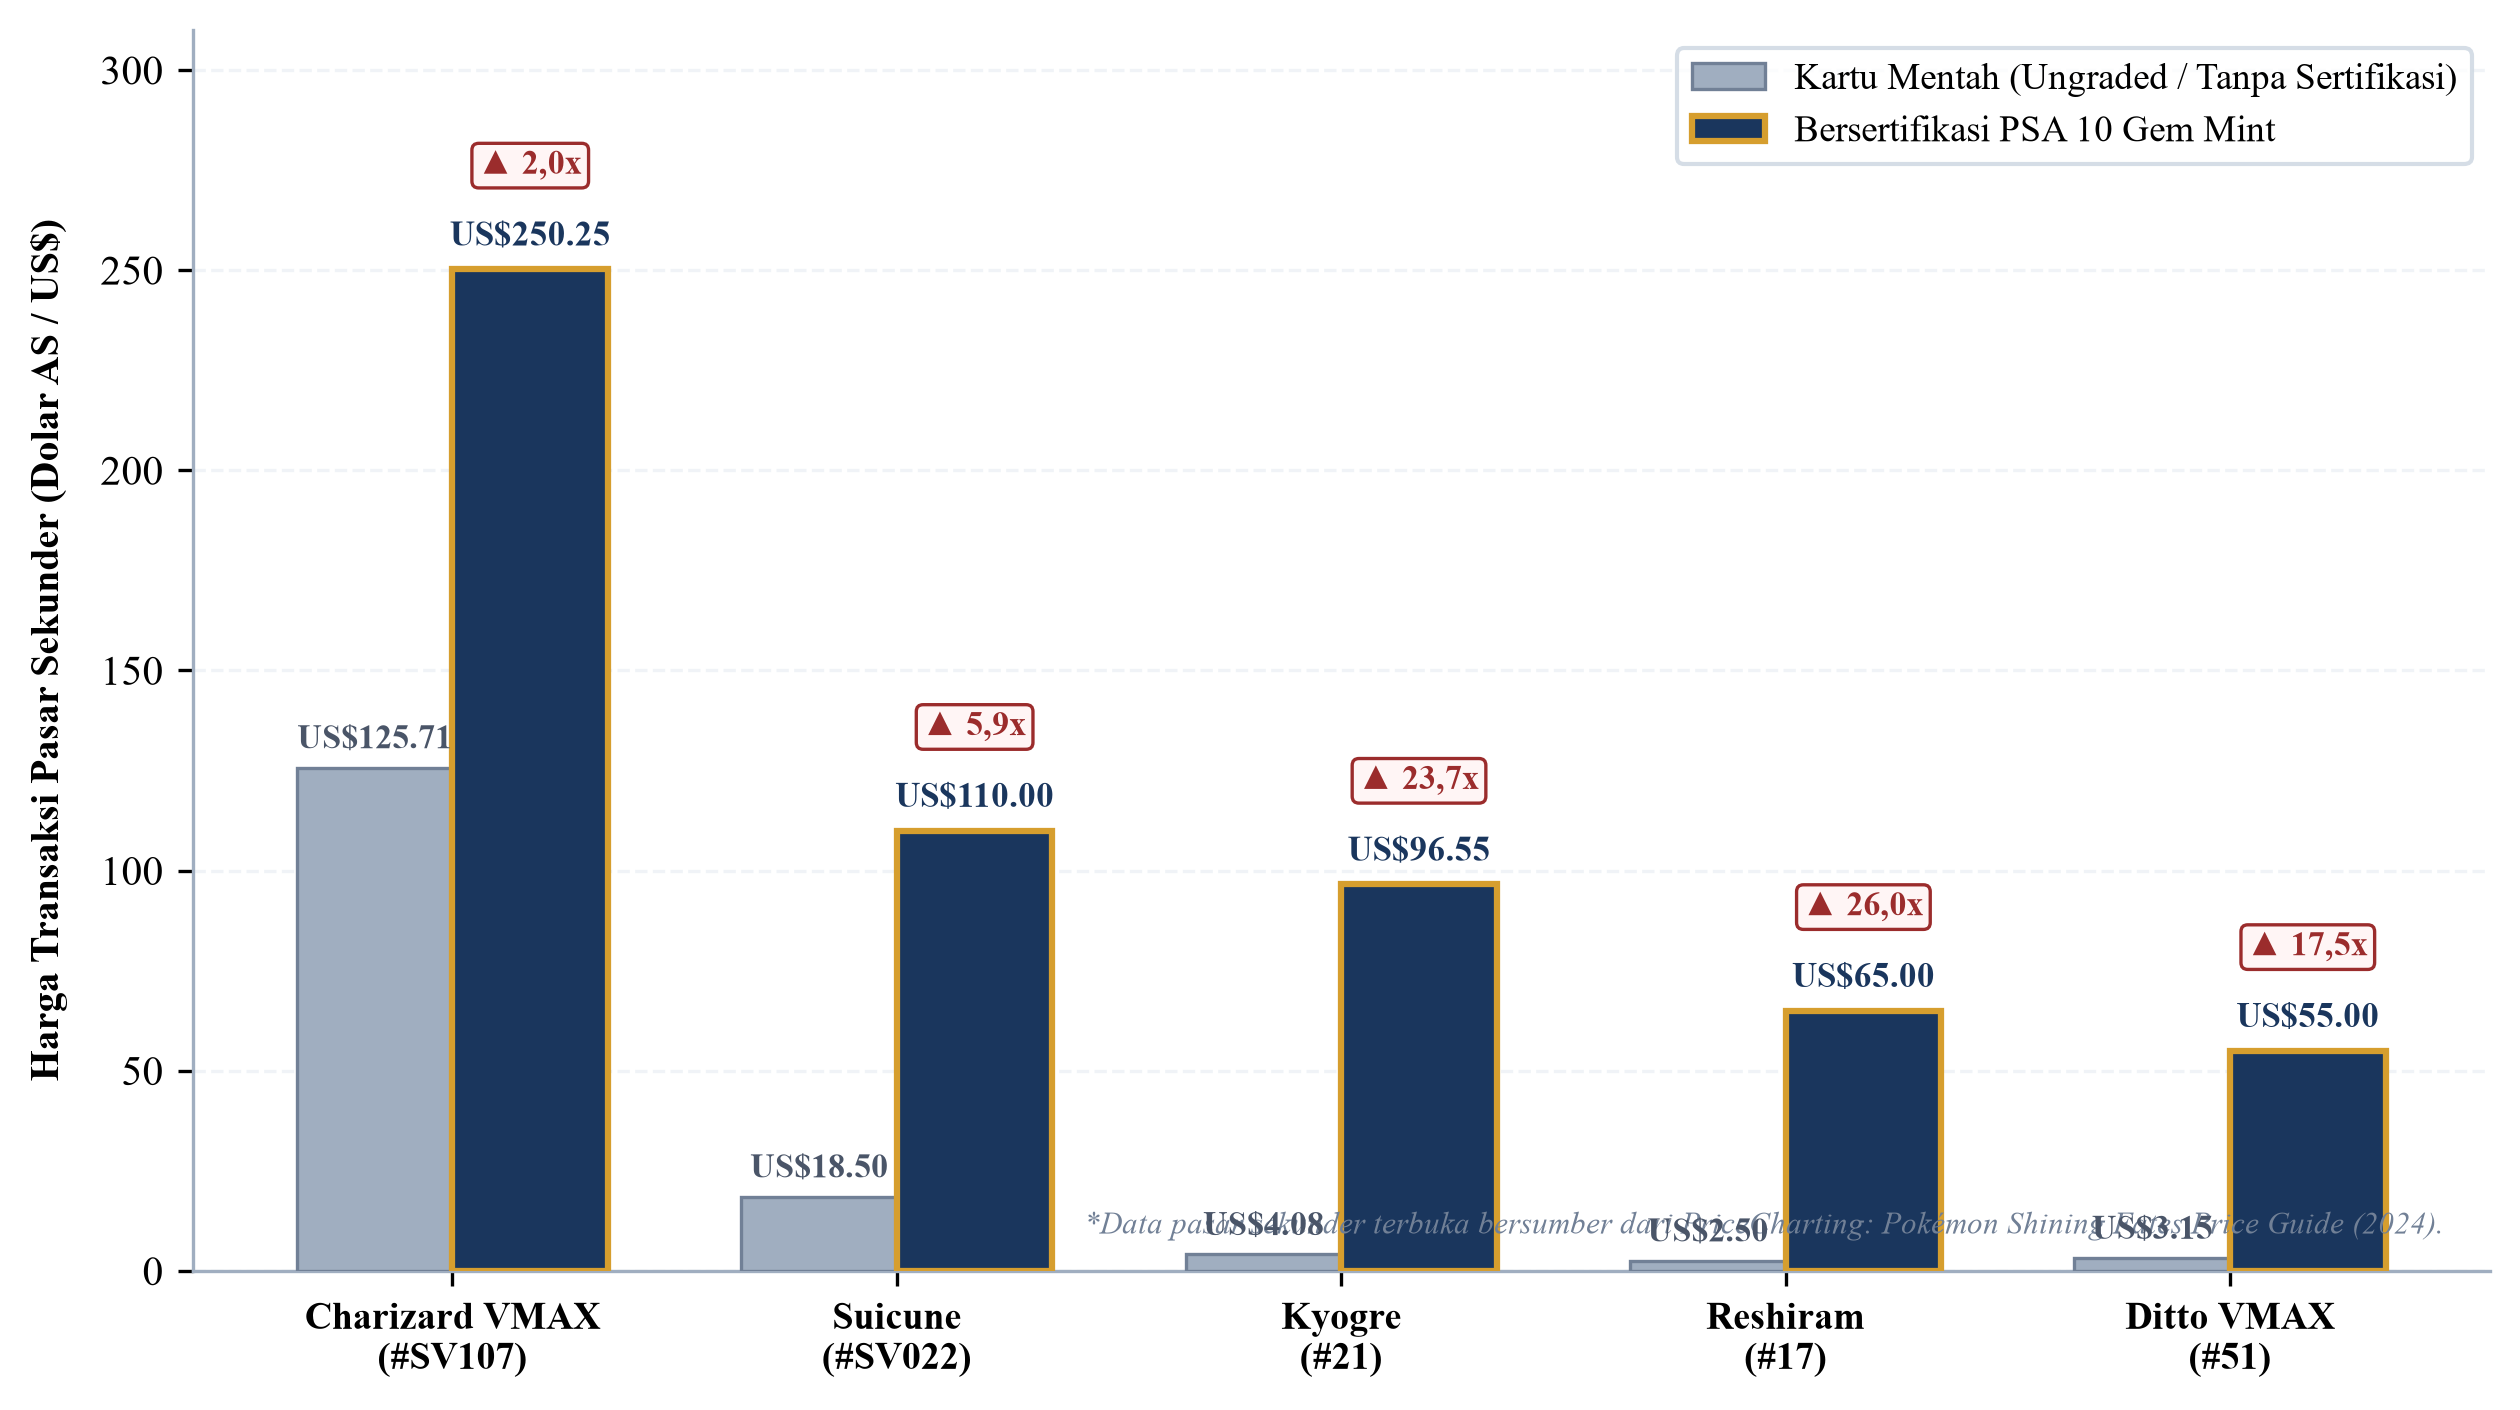
\includegraphics[width=0.80\textwidth]{images/gambar1_3_psa_grading_price_disparity.png}
  \caption{Disparitas Harga Pasar Sekunder Kartu Pok\'emon Mentah (\emph{Ungraded}) vs. Bersertifikasi \emph{PSA 10 Gem Mint} Seri \emph{Shining Fates}}
  \label{fig:pricecharting_disparity}
  \vspace{0.1cm}
  {\footnotesize \textit{Sumber: PriceCharting Market Database -- Pok\'emon Shining Fates Price Guide \citep{pricecharting2024}}\par}
\end{figure}

Sebagaimana disajikan pada Gambar 1.3, kartu berkondisi sempurna (\emph{PSA 10 Gem Mint}) mengalami apresiasi nilai pasar sekunder yang spektakuler, berkisar antara 2,0 kali lipat pada kartu langka utama (\emph{Charizard VMAX \#SV107}) hingga menembus 23,7 kali lipat (\emph{Kyogre \#21}) dan 26,0 kali lipat (\emph{Reshiram \#17}) dibandingkan kondisi kartu mentah tanpa sertifikasi \citep{pricecharting2024}. Fenomena disparitas harga yang masif ini mengilustrasikan plausibilitas bekerjanya motif spekulasi finansial (\emph{Speculative Motive} / $X_3$) di mana konsumen terdorong membeli \emph{booster pack} acak demi mengejar potensi keuntungan arbitrase \emph{grading} (\emph{grading arbitrage}). Data ini bersifat ilustratif deskriptif (bukan uji kausal $X_3$ terhadap $Y$): snapshot PriceCharting seri \emph{Shining Fates} (edisi Inggris, $N=5$ kartu contoh, diakses Januari 2025; \emph{ungraded}=harga pasar kartu mentah, \emph{PSA 10}=harga lelang kartu bersertifikasi \emph{Gem Mint}; harga volatil dan dapat berubah). Transferabilitas ke pack Indonesia berbahasa Indonesia dinyatakan sebagai keterbatasan; sebagai jembatan domestik, pola disparitas searah teramati pada listing Tokopedia/Shopee dan lelang Facebook Indonesia (tanpa generalisasi angka). \emph{Catatan kaki Gambar 1.3: snapshot Januari 2025, $N=5$ kartu Shining Fates, definisi ungraded vs PSA 10 di atas, harga volatil, bukan estimasi nasional.}

Disparitas nilai yang ekstrem dan mekanisme kemasan acak berbasis probabilitas tersebut mendorong transaksi berlebihan: setiap seri baru diluncurkan, gerai diserbu antrean dan produk ludes dalam waktu singkat, sementara pembeli membeli \emph{booster pack} berulang kali secara mendadak di kasir tanpa perencanaan anggaran. Paradoksnya, harga eceran yang terjangkau (Rp20.000--Rp30.000) dipersepsikan sebagai pengeluaran kecil yang aman, padahal isi kemasan berpeluang menjadi kartu jutaan rupiah setelah \emph{grading}. Konsumen yang semula hanya berbelanja kebutuhan harian terstimulasi menambah bungkus kartu ke keranjang semata karena letupan emosional, penasaran merobek kemasan, dan harapan spekulatif. Pola inilah gejala \textbf{pembelian impulsif (\emph{impulsive buying})} pada kartu Pok\'emon fisik di Indonesia.

Melihat fenomena tersebut, penelitian ini membedah faktor penentu pembelian impulsif kartu Pok\'emon TCG fisik di Indonesia dalam kerangka manajemen keuangan perilaku (\emph{Behavioral Finance}). Kebaruan (\emph{novelty}) penelitian ini tiga hal:
\begin{enumerate}
  \item \textbf{Komoditas hibrida:} Riset terdahulu umumnya meneliti busana, makanan, atau belanja daring umum. Penelitian ini mengkaji kartu fisik koleksi berlisensi resmi yang memiliki pasar sekunder likuid terstandardisasi (\emph{PSA 10 Gem Mint}).
  \item \textbf{Tiga dorongan sekaligus:} Riset terdahulu umumnya menguji satu dimensi. Penelitian ini mengintegrasikan motivasi hedonis (\emph{Hedonic Motivation} / $X_1$), hasrat melengkapi himpunan (\emph{Desire for Completeness} / $X_2$), dan motif spekulasi finansial (\emph{Speculative Motive} / $X_3$) dalam satu model.
  \item \textbf{Moderasi kontrol diri:} Berbeda dari studi yang menempatkan variabel psikologis sebagai prediktor langsung atau mediator, penelitian ini memposisikan \textbf{\emph{Self-Control}} sebagai \textbf{pemoderasi} yang diprediksi memperlemah pengaruh ketiga dorongan tersebut terhadap desakan belanja impulsif.
\end{enumerate}

Literatur menunjukkan pembelian impulsif dipengaruhi anteseden luas \citep{stern1962significance, rook1987buying, beatty1998impulse, amos2014meta}: (1) afektif, seperti motivasi belanja hedonis \citealp{babin1994work, arnold2003hedonic, gueltekin2012influence}; (2) kognitif kolektor, seperti efek ketidaktuntasan himpunan \citep{zeigarnik1927behalten, gao2014completing, barasz2017pseudo, belk1995collecting}; (3) finansial, seperti ekspektasi \emph{capital gain} dan bias optimisme pasar \citep{shiller2000irrational, baur2018bitcoin, colline2024biases}; serta (4) situasional, seperti display kasir dan kelangkaan stok \citep{peck2006if, amos2014meta}.

Dari pemetaan tersebut, penelitian ini memfokuskan tiga variabel yang paling mewakili karakteristik kartu Pok\'emon TCG: $X_1$ (afektif: sensasi hiburan merobek kemasan), $X_2$ (kolektor: ketegangan slot binder yang kosong), dan $X_3$ (pasar: harapan \emph{capital gain} dari likuiditas sekunder dan \emph{grading}). Perumusan instrumen dan pengujiannya diuraikan pada Bab 2 dan Bab 3.

Telaah empiris menunjukkan hubungan anteseden dengan pembelian impulsif tidak berlangsung seragam: temuan antarstudi saling bertolak belakang pada tujuh subjek hubungan dalam model ini, yakni tiga pengaruh langsung ($X_1$, $X_2$, $X_3$ terhadap $Y$), satu pengaruh langsung $M$ terhadap $Y$, dan tiga peran moderasi $M$. Pola perbedaannya konsisten secara teoretis: anggaran ketat meredam dorongan hedonis, kolektor matang berbelanja terencana di pasar sekunder, kesadaran risiko menahan spekulasi, dan kapasitas regulasi diri menipis ketika stimulus memuncak. Perbandingan temuan tersebut dirangkum pada Tabel 1.1; pembahasan tiap variabel beserta hipotesisnya diuraikan pada Bab 2.

\begingroup
\footnotesize
\begin{longtable}{p{0.04\textwidth} p{0.21\textwidth} p{0.24\textwidth} p{0.24\textwidth} p{0.21\textwidth}}
\caption{Matriks Kesenjangan Penelitian Empiris (\emph{Research Gap}) pada 7 Subjek Hubungan Model Penelitian} \label{tab:research_gap} \\
\toprule
\textbf{No} & \textbf{Subjek Hubungan} & \textbf{Kelompok Temuan Positif / Meredam} & \textbf{Kelompok Temuan Negatif / Lemah} & \textbf{Inti Kesenjangan Kausal (\emph{The Why})} \\
\midrule
\endfirsthead
\toprule
\textbf{No} & \textbf{Subjek Hubungan} & \textbf{Kelompok Temuan Positif / Meredam} & \textbf{Kelompok Temuan Negatif / Lemah} & \textbf{Inti Kesenjangan Kausal (\emph{The Why})} \\
\midrule
\endhead
\midrule
\multicolumn{5}{r}{\footnotesize\textit{Bersambung ke halaman berikutnya}} \\
\endfoot
\bottomrule
\endlastfoot

1 & $X_1$ terhadap $Y$ (\emph{Hedonic Motivation}) & \citet{arnold2003hedonic}; \citet{gueltekin2012influence}; \citet{pranggabayu2022pengaruh}; \citet{gong2024unveiling}; \citet{tirtayasa2020effect}; \citet{zheng2019impact} (positif signifikan). & Batas \citet{thaler1985mental, thaler1981economic} (tertahan anggaran; bukan temuan tidak signifikan pada kolektibel). & Elastisitas anggaran dan orientasi utiliter vs afektif. \\
\addlinespace[2pt]
2 & $X_2$ terhadap $Y$ (\emph{Desire for Completeness}) & \citet{gao2014completing}; \citet{barasz2017pseudo}; \citet{dewi2026understanding} (positif signifikan). & \citet{long2000consuming}; \citet{spero2004approach} (kolektor matang pilih \emph{single}; bukan temuan tidak signifikan). & Kematangan kolektor dan kalkulasi probabilitas. \\
\addlinespace[2pt]
3 & $X_3$ terhadap $Y$ (\emph{Speculative Motive}) & \citet{baur2018bitcoin}; \citet{aryadi2024personal} (analogi partisipasi TCG); \citet{colline2024biases} (herding; kualitatif); \citet{shiller2000irrational} sebagai \emph{grand theory}. & \citet{barber2008all}; \citet{fama1970efficient} (analogi saham; bukan temuan tidak signifikan pada kolektibel). & Asimetri informasi dan ilusi kendali vs evaluasi risiko. \\
\addlinespace[2pt]
4 & $M$ terhadap $Y$ (\emph{Self-Control}) & \citet{baumeister2002yield}; \citet{tangney2004high}; \citet{vohs2007spent}; \citet{sultan2012building} (negatif signifikan). & \citet{hirschman1982hedonic}; \citet{stern1962significance} (\emph{cognitive bypass}; bukan regresi). & \emph{Ego depletion} saat stimulus intens. \\
\addlinespace[2pt]
5 & Moderasi $M$ pada $X_1$ terhadap $Y$ & \citet{lienardy2026role} (MRA H4 diterima); \citet{katauke2023financial} (tak langsung). & Gagal-moderasi \citet{apidana2022peran} (p=0,597) dan \citet{artadita2024how} ($\beta=0{,}092$, tidak signifikan) + \emph{regulatory failure}. & Ambang intensitas hedonis vs kapasitas volisional. \\
\addlinespace[2pt]
6 & Moderasi $M$ pada $X_2$ terhadap $Y$ & Parsial: \citet{artadita2024how} (kontrol kognitif; moderasi keseluruhan ditolak); \citet{apidana2022peran} (adjacent). & Teori \citet{belk1995collecting}; \citet{barasz2017pseudo} + \citet{artadita2024how} H3 ditolak. & Keterikatan koleksi: kasual vs fanatik. \\
\addlinespace[2pt]
7 & Moderasi $M$ pada $X_3$ terhadap $Y$ & Tak langsung: \citet{katauke2023financial} + \emph{Planner-Doer}. & Teoritis \citet{shiller2000irrational}; \citet{aryadi2024personal} (bukan uji interaksi). & \emph{Herding} dan FOMO saat euforia. \\
\end{longtable}
\vspace{-0.3cm}
\begin{flushleft}
  \footnotesize\textit{Sumber: Data diolah dari sintesis kajian literatur empiris terdahulu (2026).}
\end{flushleft}
\endgroup

Ketidakseragaman temuan tersebut menunjukkan perlunya variabel pemoderasi yang menguji batas kontrol psikologis konsumen. Dalam kerangka \emph{Self-Regulation Theory} \citep{baumeister2002yield, vohs2007spent} dan model \emph{Planner-Doer} \citep{thaler1981economic}, \textbf{\emph{Self-Control}} diposisikan sebagai rem volisional, yakni kapasitas menunda kepuasan \citep{tangney2004high, sultan2012building} yang diprediksi \textbf{memperlemah} ketiga dorongan tersebut \citep{lienardy2026role}.

Berdasarkan latar belakang permasalahan, urgensi empiris, dan kebaruan konseptual tersebut, penelitian ini memiliki orisinalitas tinggi dalam ranah manajemen keuangan perilaku dan perilaku konsumen di Indonesia. Berlandaskan seluruh uraian di atas, peneliti menetapkan judul skripsi: \textbf{``\judulskripsi''}.

\subsection{Perumusan Masalah}

Berdasarkan latar belakang penelitian yang telah diuraikan, maka perumusan masalah dalam penelitian ini adalah sebagai berikut:
\begin{enumerate}
  \item Apakah \emph{Hedonic Motivation} berpengaruh terhadap \emph{Impulsive Buying} \emph{booster pack} kartu Pok\'emon TCG?
  \item Apakah \emph{Desire for Completeness} berpengaruh terhadap \emph{Impulsive Buying} \emph{booster pack} kartu Pok\'emon TCG?
  \item Apakah \emph{Speculative Motive} berpengaruh terhadap \emph{Impulsive Buying} \emph{booster pack} kartu Pok\'emon TCG?
  \item Apakah \emph{Self-Control} memoderasi (memperlemah) pengaruh \emph{Hedonic Motivation} terhadap \emph{Impulsive Buying} \emph{booster pack} kartu Pok\'emon TCG?
  \item Apakah \emph{Self-Control} memoderasi (memperlemah) pengaruh \emph{Desire for Completeness} terhadap \emph{Impulsive Buying} \emph{booster pack} kartu Pok\'emon TCG?
  \item Apakah \emph{Self-Control} memoderasi (memperlemah) pengaruh \emph{Speculative Motive} terhadap \emph{Impulsive Buying} \emph{booster pack} kartu Pok\'emon TCG?
\end{enumerate}

\subsection{Tujuan Penelitian}

Mengacu pada perumusan masalah di atas, maka tujuan yang ingin dicapai dalam penelitian ini adalah:
\begin{enumerate}
  \item Untuk menganalisis dan membuktikan secara empiris pengaruh \emph{Hedonic Motivation} terhadap \emph{Impulsive Buying} \emph{booster pack} kartu Pok\'emon TCG.
  \item Untuk menganalisis dan membuktikan secara empiris pengaruh \emph{Desire for Completeness} terhadap \emph{Impulsive Buying} \emph{booster pack} kartu Pok\'emon TCG.
  \item Untuk menganalisis dan membuktikan secara empiris pengaruh \emph{Speculative Motive} terhadap \emph{Impulsive Buying} \emph{booster pack} kartu Pok\'emon TCG.
  \item Untuk menganalisis dan membuktikan secara empiris peran moderasi \emph{Self-Control} yang memperlemah pengaruh \emph{Hedonic Motivation} terhadap \emph{Impulsive Buying} \emph{booster pack} kartu Pok\'emon TCG.
  \item Untuk menganalisis dan membuktikan secara empiris peran moderasi \emph{Self-Control} yang memperlemah pengaruh \emph{Desire for Completeness} terhadap \emph{Impulsive Buying} \emph{booster pack} kartu Pok\'emon TCG.
  \item Untuk menganalisis dan membuktikan secara empiris peran moderasi \emph{Self-Control} yang memperlemah pengaruh \emph{Speculative Motive} terhadap \emph{Impulsive Buying} \emph{booster pack} kartu Pok\'emon TCG.
\end{enumerate}

\subsection{Manfaat Penelitian}

Hasil penelitian ini diharapkan dapat memberikan kontribusi nyata baik secara teoritis maupun praktis:

\subsubsection{Manfaat Teoritis}
\begin{enumerate}
  \item \textbf{Pengembangan Teori Keuangan Perilaku (\emph{Behavioral Finance}):} Memberikan kontribusi empiris dalam memperluas cakupan teori keuangan perilaku pada pasar aset alternatif (\emph{collectibles}), khususnya dalam menjelaskan bagaimana motif spekulasi finansial, bias perilaku investor Indonesia \citep{colline2024biases}, dan bias kognitif koleksi berinteraksi memicu keputusan pembelian impulsif.
  \item \textbf{Pengayaan Literatur Moderasi Kontrol Diri (\emph{Self-Control}):} Memperdalam pemahaman teoretis mengenai mekanisme regulasi diri (\emph{Self-Regulation Theory}) dalam memoderasi dan meredam dorongan belanja spontan pada barang-barang berkategori kesenangan dan spekulasi hobi \citep{sultan2012building, apidana2022peran, lienardy2026role}.
  \item \textbf{Referensi Akademis Baru:} Menjadi rujukan ilmiah pionir bagi penelitian-penelitian di masa depan di lingkungan Fakultas Ekonomi dan Bisnis terkait perilaku konsumen dan dinamika ekonomi industri \emph{Trading Card Game} di Indonesia yang selama ini masih sangat jarang diteliti.
\end{enumerate}

\subsubsection{Manfaat Praktis}
\begin{enumerate}
  \item \textbf{Bagi Konsumen dan Kolektor Pok\'emon TCG:} Memberikan kesadaran kritis dan evaluasi diri bagi para kolektor (khususnya mahasiswa dan Generasi Z) agar lebih mengenali bias emosional dan ilusi spekulasi finansial dalam hobi kartu, sehingga mampu mengoptimalkan kontrol diri dan menjaga kesehatan keuangan pribadi.
  \item \textbf{Bagi Komunitas dan Pelaku Usaha Toko Hobi (\emph{Local Game Stores}):} Menjadi referensi wawasan perilaku konsumen bagi pengelola toko dan komunitas permainan kartu agar dapat membangun ekosistem komunitas yang sehat, edukatif, dan berkelanjutan tanpa mengeksploitasi dorongan impulsif pembeli secara destruktif.
  \item \textbf{Bagi Otoritas Edukasi Finansial dan Kebijakan Publik:} Memberikan data dan fakta lapangan mengenai pola pengeluaran konsumtif berbasis probabilitas dan spekulasi pada kalangan generasi muda, yang berguna sebagai bahan pertimbangan dalam merancang materi pengendalian diri finansial yang kontekstual bagi Generasi Z.
  \item \textbf{Bagi Almamater FEB UKRIDA:} Menambah koleksi karya ilmiah berkualitas dan orisinal di Program Studi S1 Manajemen Konsentrasi Manajemen Keuangan Fakultas Ekonomi dan Bisnis Universitas Kristen Krida Wacana.
\end{enumerate}

% ============================================================
%  BAB 2: KAJIAN PUSTAKA DAN PENGEMBANGAN HIPOTESIS
% ============================================================
\newpage
\setcounter{section}{1}
\section*{BAB 2\\[0.3cm]KAJIAN PUSTAKA DAN PENGEMBANGAN HIPOTESIS}
\addcontentsline{toc}{section}{\texorpdfstring{BAB 2\quad KAJIAN PUSTAKA DAN PENGEMBANGAN HIPOTESIS}{BAB 2 KAJIAN PUSTAKA DAN PENGEMBANGAN HIPOTESIS}}
\setcounter{section}{2}
\setcounter{subsection}{0}
\setcounter{table}{0}
\setcounter{figure}{0}
\setcounter{equation}{0}

\subsection{Landasan Teori}

\subsubsection{Grand Theory: Keuangan Perilaku (\emph{Behavioral Finance})}

Teori utama (\emph{grand theory}) yang dipakai adalah \textbf{Keuangan Perilaku (\emph{Behavioral Finance})}. Teori keuangan neoklasik tradisional berasumsi bahwa pelaku ekonomi merupakan makhluk yang sepenuhnya rasional (\emph{homo economicus}) yang selalu memaksimalkan utilitas dan memproses informasi secara efisien \citep{fama1970efficient}. Namun, \citet{simon1955behavioral} mengemukakan konsep rasionalitas terbatas (\emph{bounded rationality}), bahwa keterbatasan kapasitas kognitif dan informasi membuat manusia tidak mampu mengambil keputusan yang optimal sempurna, melainkan memilih alternatif yang memuaskan (\emph{satisficing}).

\citet{kahneman1979prospect} melalui \emph{Prospect Theory} membuktikan bahwa individu mengevaluasi keuntungan dan kerugian secara asimetris (\emph{loss aversion}), serta dipandu oleh bias kognitif sistematis seperti \emph{overoptimism bias} dan kesesatan berpikir penjudi (\emph{gambler's fallacy / lottery effect}). \citet{shiller2000irrational} dalam \emph{Irrational Exuberance} menguraikan bagaimana dinamika psikologis pasar dan perilaku berkerumun (\emph{herd behavior}) memicu gelembung spekulatif (\emph{speculative bubbles}) di mana harga aset melonjak jauh melampaui nilai fundamentalnya. Selanjutnya, \citet{thaler1985mental} dan \citet{thaler1981economic} memperkenalkan konsep \emph{Mental Accounting} serta model konflik internal dua sistem (\emph{Dual-System Planner-Doer Model}): pertarungan antara entitas perencana (\emph{planner}) yang rasional jangka panjang dengan entitas pelaku (\emph{doer}) yang impulsif jangka pendek.

Dalam konteks kartu Pok\'emon TCG, \emph{Behavioral Finance} memberikan landasan eksplanatif yang solid. Kartu Pok\'emon fisik telah bertransformasi menjadi instrumen aset alternatif yang sarat dengan bias perilaku keuangan: ilusi probabilitas menarik kartu \emph{Gem Mint 10} bernilai jutaan rupiah dari kemasan murah, godaan kepuasan instan merobek bungkus kemasan, serta antusiasme spekulatif yang mengabaikan ketersediaan anggaran pribadi.

\subsubsection{Supporting Theory: Teori \emph{Stimulus-Organism-Response} (S-O-R)}

Model \emph{Stimulus-Organism-Response} (S-O-R) dari \citet{mehrabian1974approach} menjadi kerangka pendukung. Model ini menjelaskan bahwa pemicu lingkungan eksternal (\emph{Stimulus}) mempengaruhi kondisi internal kognitif dan afektif individu (\emph{Organism}), yang pada gilirannya memicu tindakan nyata (\emph{Response}):
\begin{enumerate}
  \item \textbf{Stimulus (S):} Pajangan kemasan \emph{booster pack} di kasir minimarket, mekanisme kejutan bungkus acak (\emph{blind-pack}), promosi rilis seri baru, serta dinamika harga mahal di pasar sekunder.
  \item \textbf{Organism (O):} Kondisi emosional mencari kesenangan (\emph{Hedonic Motivation} / $X_1$), desakan psikologis menutup slot album (\emph{Desire for Completeness} / $X_2$), motif spekulasi keuntungan modal (\emph{Speculative Motive} / $X_3$), serta kapasitas pengaturan diri sebagai pemoderasi (\emph{Self-Control} / $M$).
  \item \textbf{Response (R):} Tindakan akhir berupa pembelian spontan dan tidak terencana (\emph{Impulsive Buying} / $Y$).
\end{enumerate}

\subsubsection{Supporting Theory: Psikologi Kolektor dan \emph{Collection-Goal Tipping Point Effect}}

Mengoleksi adalah bentuk konsumsi aktif dan penuh gairah yang didorong oleh kebutuhan psikologis akan keteraturan dan pencapaian \citep{belk1995collecting}. Dorongan ini berakar pada \emph{Zeigarnik Effect} \citep{zeigarnik1927behalten}, di mana tugas atau susunan yang belum lengkap menghasilkan ketegangan kognitif internal (\emph{cognitive tension}) yang menuntut penyelesaian (\emph{closure}). \citet{gao2014completing} dalam studi seminalnya di \emph{Journal of Marketing} memformalkan fenomena ini sebagai \textbf{\emph{collection-goal tipping point effect}}, menunjukkan bahwa motivasi konsumen mengakuisisi barang menguat saat set mendekati kelengkapan. \citet{barasz2017pseudo} memperkuat temuan ini melalui konsep \textbf{\emph{Pseudo-Set Framing}}, di mana pembeli terdorong melengkapi item yang dibingkai sebagai kesatuan himpunan utuh.

\subsubsection{Supporting Theory: Teori Regulasi Diri (\emph{Self-Regulation Theory})}

Teori regulasi diri \citep{baumeister2002yield} menjelaskan bagaimana individu mengendalikan dorongan instingtual demi tujuan jangka panjang. \citet{vohs2007spent} membuktikan bahwa penipisan kontrol diri secara langsung menyebabkan kegagalan menahan impuls belanja. Sebaliknya, individu dengan kontrol diri yang kuat (\emph{high trait self-control}) memiliki kapasitas volisional tangguh untuk menolak godaan belanja sesaat dan menunda kepuasan (\emph{delay of gratification}) \citep{tangney2004high}.

\subsection{Kajian Variabel Penelitian}

\subsubsection{Variabel Dependen ($Y$): \emph{Impulsive Buying} (Pembelian Impulsif)}

Pembelian impulsif didefinisikan sebagai dorongan belanja mendadak, kuat, dan persisten untuk segera bertransaksi tanpa adanya deliberasi kognitif sadar sebelumnya mengenai konsekuensi pengeluaran \citep{stern1962significance, rook1987buying, rook1995normative}. \citet{verplanken2001individual} mengidentifikasi dua dimensi utama: (1) dimensi kognitif (ketiadaan perencanaan dan pengabaian anggaran); dan (2) dimensi afektif (luapan kegembiraan dan dorongan emosional tak tertahankan). \citet{amos2014meta} menegaskan bahwa pembelian impulsif dipicu oleh konvergensi stimulus afektif, faktor kognitif internal, dan situasi pasar.

\subsubsection{Variabel Independen ($X_1$): \emph{Hedonic Motivation} (Motivasi Hedonis)}

Motivasi hedonis merujuk pada dorongan berbelanja demi kesenangan emosional, hiburan, dan pengalaman multisensori, bukan semata kegunaan utiliter \citep{hirschman1982hedonic, babin1994work}. \citet{arnold2003hedonic} merumuskan enam dimensi motivasi hedonis, di mana dimensi \emph{Adventure Shopping} (sensasi petualangan dan kejutan) serta \emph{Gratification Shopping} (pelepasan stres dan hadiah diri) merupakan dimensi paling dominan dalam pembelian \emph{booster pack} kartu Pok\'emon TCG fisik. Dimensi keenam, \emph{Value Shopping} (perburuan harga murah), sengaja tidak diadaptasi karena harga eceran \emph{booster pack} bersifat pasti dan seragam (Rp20.000--Rp30.000), sehingga motif tawar-menawar tidak relevan; operasionalisasi memakai lima dimensi terapan (X1.1--X1.5 pada Tabel 3.2).

\subsubsection{Variabel Independen ($X_2$): \emph{Desire for Completeness} (Hasrat Kelengkapan Koleksi)}

\emph{Desire for Completeness} didefinisikan sebagai dorongan motivasional internal individu untuk melengkapi seluruh elemen dari suatu himpunan yang telah terdefinisi batasannya secara utuh \citep{belk1995collecting, gao2014completing, barasz2017pseudo}. Dimensi utamanya mencakup: persepsi batasan himpunan (\emph{perceived set boundaries}), ketegangan kognitif celah koleksi (\emph{cognitive incompletion tension}), dan desakan penuntasan himpunan (\emph{drive for closure}). Setiap seri Pok\'emon TCG memiliki nomor urut resmi; kotak slot kosong pada album \emph{binder} kolektor memicu ketegangan kognitif yang mendesak pembelian kemasan tambahan demi mengisi nomor yang hilang.

\subsubsection{Variabel Independen ($X_3$): \emph{Speculative Motive} (Motif Spekulasi Finansial)}

Motif spekulasi berakar pada teori moneter \citet{keynes1936general} dan \emph{Behavioral Finance} \citep{shiller2000irrational, baur2018bitcoin}, yaitu hasrat mengakuisisi barang dengan ekspektasi menjualnya kembali demi perolehan keuntungan modal (\emph{capital gain}). Dimensinya meliputi: ekspektasi kenaikan harga pasar, sensitivitas terhadap likuiditas pasar sekunder, dan motif arbitrase \emph{grading} (\emph{grading arbitrage}).

Kehadiran lembaga sertifikasi \emph{grading} independen internasional (\textbf{PSA, BGS, CGC}) yang menilai kondisi fisik kartu secara mikroskopis pada skala 1--10 (\emph{Gem Mint 10}) mentransformasi kartu Pok\'emon menjadi aset alternatif terstandardisasi. Kartu bergradasi \emph{PSA 10 Gem Mint} memiliki likuiditas lelang global dan harga jual yang melonjak hingga puluhan kali lipat dibandingkan kartu mentah (\emph{raw card}), sehingga menjadi katalisator pemicu motif spekulasi finansial pembeli.

\subsubsection{Variabel Moderasi ($M$): \emph{Self-Control} (Kontrol Diri)}

Kontrol diri merupakan kapasitas volisional individu untuk menolak godaan belanja, menunda kepuasan sesaat (\emph{delay of gratification}), dan mendisiplinkan pengeluaran agar selaras dengan rencana keuangan jangka panjang \citep{tangney2004high, baumeister2002yield, vohs2007spent}. Dalam model \emph{Planner-Doer} \citep{thaler1981economic}, kontrol diri bertindak sebagai rem volisional kognitif. Konsumen dengan kontrol diri tinggi mampu menahan desakan emosional dan spekulatif, sehingga pengaruh variabel independen terhadap \emph{Impulsive Buying} diperlemah secara signifikan \citep{sultan2012building}.

\subsection{Penelitian Sebelumnya}

Berikut disajikan ringkasan sepuluh studi empiris 2021--2026 yang menopang perumusan hipotesis H1--H6:

\begingroup
\singlespacing
\setlength{\tabcolsep}{4pt}
\small
\begin{longtable}{>{\centering\arraybackslash}p{0.5cm} >{\raggedright\arraybackslash}p{2.3cm} >{\raggedright\arraybackslash}p{3.2cm} >{\raggedright\arraybackslash}p{2.6cm} >{\raggedright\arraybackslash}p{3.9cm}}
\caption{Ringkasan Penelitian Sebelumnya} \label{tab:penelitian_terdahulu} \\
\toprule
\textbf{No} & \textbf{Peneliti (Tahun)} & \textbf{Judul Penelitian} & \textbf{Variabel \& Metode} & \textbf{Hasil Utama} \\
\midrule
\endfirsthead
\multicolumn{5}{l}{\footnotesize\textit{Lanjutan Tabel \thetable\ -- Ringkasan Penelitian Sebelumnya}} \\[0.2cm]
\toprule
\textbf{No} & \textbf{Peneliti (Tahun)} & \textbf{Judul Penelitian} & \textbf{Variabel \& Metode} & \textbf{Hasil Utama} \\
\midrule
\endhead
\midrule
\multicolumn{5}{r}{\footnotesize\textit{Bersambung ke halaman berikutnya}} \\
\endfoot
\bottomrule
\endlastfoot

1 & \citet{pranggabayu2022pengaruh} & Pengaruh \emph{Hedonic Shopping Motivation} dan \emph{Store Atmosphere} terhadap \emph{Impulsive Buying} & X1: \emph{Hedonic shopping motivation}, X2: \emph{Store atmosphere}; Y: \emph{Impulsive buying}; Regresi linear berganda (200 responden) & Motivasi belanja hedonis terbukti mendorong \emph{impulsive buying}; kesenangan berbelanja menurunkan deliberasi rasional konsumen. \\
\addlinespace[4pt]
2 & \citet{apidana2022peran} & Peran \emph{Self-Control} dalam Memoderasi Pengaruh \emph{Hedonic Motives} dan \emph{Shopping Lifestyle} terhadap \emph{Impulse Buying} & X1: \emph{Hedonic motives}, X2: \emph{Shopping lifestyle}; Y: \emph{Impulse buying}; Mod: \emph{Self-control}; MRA & Motif hedonis positif signifikan; kontrol diri memoderasi \emph{shopping lifestyle} (H4 diterima, $\beta<0$) tetapi GAGAL memoderasi \emph{hedonic motives} (H3 ditolak, p=0,597). \\
\addlinespace[4pt]
3 & \citet{lienardy2026role} & \emph{The Role of Self-Control in Moderating the Influence of Shopping Lifestyle and Hedonistic Behavior on Impulsive Buying} & X1: \emph{Shopping lifestyle}, X2: \emph{Hedonistic behavior}; Y: \emph{Impulsive buying}; Mod: \emph{Self-control}; MRA (160 responden) & Perilaku hedonis menunjukkan hubungan positif yang signifikan dengan pembelian impulsif; kontrol diri terbukti memoderasi dan memperlemah pengaruh perilaku hedonis terhadap \emph{impulsive buying}. \\
\addlinespace[4pt]
4 & \citet{gong2024unveiling} & \emph{Unveiling the Enigma of Blind Box Impulse Buying Curiosity: The Moderating Role of Price Consciousness} & X: Karakteristik kemasan \emph{blind box}; Med: Rasa ingin tahu; Y: \emph{Impulse buying}; Kerangka S-O-R; PLS-SEM (306 responden) & Mekanisme kejutan kemasan tertutup (\emph{blind box/booster pack}) memicu rasa ingin tahu afektif yang secara langsung mendorong pembelian impulsif; kesadaran harga memoderasi hubungan tersebut. \\
\addlinespace[4pt]
5 & \citet{azizah2025exploring} & Pengaruh \emph{Hedonic Motivation}, \emph{Shopping Lifestyle}, dan \emph{Positive Emotions} terhadap \emph{Impulse Buying} & X1: \emph{Hedonic motivation}, X2: \emph{Shopping lifestyle}; Med: \emph{Positive emotions}; Y: \emph{Impulse buying}; PLS-SEM, survei e-commerce fashion Indonesia (n=140 purposive) & Motivasi hedonis tercatat berpengaruh positif dan signifikan terhadap pembelian impulsif; emosi positif memediasi parsial dan menjadi jalur terkuat. Bukti domestik terkini untuk H1. \\
\addlinespace[4pt]
6 & \citet{dewi2026understanding} & \emph{Understanding Impulse Buying Behavior: The Case of Blind Box Purchases in Indonesia} & X1: \emph{Perceived scarcity}, X2: \emph{Perceived uncertainty}; Med: FOMO; Y: \emph{Impulse buying}; PLS-SEM (211 Gen Z Indonesia) & Persepsi kelangkaan item dan ketidakpastian memicu FOMO dan hasrat memiliki set koleksi utuh, yang secara langsung dan signifikan memicu \emph{impulse buying} pada Generasi Z di Indonesia. \\
\addlinespace[4pt]
7 & \citet{aryadi2024personal} & \emph{Personal Traits and Motivation Impact on Collectibles as an Alternative Investment: A Case Study of Trading Card Game Community in Greater Jakarta} & X: Motivasi kolektor \& ciri kepribadian; Y: Keputusan investasi TCG; Regresi logistik biner (158 anggota komunitas TCG) & Membuktikan bahwa motivasi kolektor dan motif spekulasi finansial secara positif mendorong partisipasi dalam transaksi kartu TCG (Pok\'emon, dkk.) sebagai aset alternatif investasi di Jabodetabek. \\
\addlinespace[4pt]
8 & \citet{colline2024biases} & \emph{Biases in Indonesian Stock Investor Behavior} & X: Bias perilaku (\emph{herding}, \emph{loss aversion}); Y: Keputusan investasi; Kualitatif wawancara mendalam (n=5 investor Indonesia) & Mendokumentasikan kuatnya \emph{herding} (ikut-ikutan), \emph{loss aversion}, dan \emph{disposition effect} pada investor Indonesia, dipakai sebagai analogi bias pasar aset. \\
\addlinespace[4pt]
9 & \citet{artadita2024how} & \emph{How Does Self-Control Moderate Shopping Enjoyment and Impulse Buying Among Generation Z Online Gamers?} & X: Kenikmatan belanja (\emph{shopping enjoyment}); Y: \emph{Impulse buying}; Mod: \emph{Self-control}; PLS-SEM + regresi dimensional (220 Gen Z Gamers; bukan MRA) & Kenikmatan belanja berpengaruh positif kuat ($\beta=0{,}581$); efek moderasi kontrol diri DITOLAK ($\beta=0{,}092$) kecuali dimensi kontrol kognitif yang signifikan pada taraf 10\% (p$<0{,}10$). \\
\addlinespace[4pt]
10 & \citet{katauke2023financial} & \emph{Financial Literacy and Impulsivity: Evidence from Japan} & X: Literasi finansial; Y: \emph{Impulsivity (hyperbolic discounting)}; Probit + \emph{instrumental variables} & Literasi finansial berhubungan negatif dengan diskonto hiperbolik (proksi impulsivitas); bukti regulasi-rasional dari Jepang. \\
\end{longtable}
\vspace{-0.3cm}
\begin{flushleft}
  \footnotesize\textit{Sumber: Data diolah dari publikasi jurnal ilmiah bereputasi 2021--2026 (2026).}
\end{flushleft}
\endgroup

\subsection{Pengembangan Hipotesis}

\subsubsection{Pengaruh \emph{Hedonic Motivation} terhadap \emph{Impulsive Buying}}

\noindent\textbf{Landasan Teoretis:} Model S-O-R \citep{mehrabian1974approach} dan teori konsumsi pengalaman \citep{hirschman1982hedonic} memposisikan belanja sebagai sarana mencari kesenangan emosional dan fantasi. Rangsangan afektif ini menurunkan pertimbangan rasional dan mendorong tindakan belanja seketika demi mempertahankan suasana hati positif \citep{babin1994work}.

\noindent\textbf{Kajian Empiris Terdahulu:} Bukti empiris terkini dari \citet{pranggabayu2022pengaruh}, \citet{azizah2025exploring}, serta \citet{artadita2024how} pada konsumen Indonesia menunjukkan bahwa motivasi hedonis dan kenikmatan berbelanja (\emph{shopping enjoyment}) berpengaruh positif signifikan terhadap perilaku \emph{impulsive buying}.

\noindent\textbf{Keterkaitan dengan Objek (Pok\'emon TCG):} Kemasan tertutup \emph{booster pack} menghadirkan elemen kejutan mendebarkan. Sensasi merobek kemasan foil dan sensasi puas yang intens saat mendapati kartu hologram langka memberikan kenikmatan emosional instan. Akibatnya, pembelian berulang terjadi secara mendadak di kasir toko tanpa perencanaan anggaran.

\vspace{0.2cm}
\textbf{H1: \emph{Hedonic Motivation} berpengaruh positif dan signifikan terhadap \emph{Impulsive Buying} \emph{booster pack} kartu Pok\'emon TCG.}

\subsubsection{Pengaruh \emph{Desire for Completeness} terhadap \emph{Impulsive Buying}}

\noindent\textbf{Landasan Teoretis:} Titik berangkatnya adalah \emph{Zeigarnik Effect} \citep{zeigarnik1927behalten} dan \emph{collection-goal tipping point effect} \citep{gao2014completing}: manusia memiliki resistensi alami terhadap ketidaktuntasan (\emph{aversion to incompleteness}). Celah dalam suatu himpunan menciptakan ketegangan kognitif yang mendesak tindakan penyelesaian \citep{belk1995collecting, barasz2017pseudo}.

\noindent\textbf{Kajian Empiris Terdahulu:} Selain temuan seminal \citet{gao2014completing}, riset empiris mutakhir pada produk berkemasan acak (\emph{blind-box}) oleh \citet{gong2024unveiling} (responden China) serta \citet{dewi2026understanding} (Generasi Z Indonesia) menunjukkan bahwa mekanisme kejutan kemasan, persepsi kelangkaan (\emph{scarcity}), dan hasrat menuntaskan seri koleksi menjadi pemicu pembelian impulsif yang agresif pada Generasi Z; bukti domestik Indonesia ditopang oleh \citet{dewi2026understanding}.

\noindent\textbf{Keterkaitan dengan Objek (Pok\'emon TCG):} Setiap seri kartu Pok\'emon dirilis dengan daftar periksa (\emph{set checklist}) bernomor urut resmi. Kotak slot kosong pada album \emph{binder} kolektor memicu ketegangan kognitif visual yang kuat untuk menuntaskan set secara utuh. Desakan menutup celah kosong ini membuat kolektor membeli \emph{booster pack} secara terburu-buru dan spontan saat berada di toko ritel.

\vspace{0.2cm}
\textbf{H2: \emph{Desire for Completeness} berpengaruh positif dan signifikan terhadap \emph{Impulsive Buying} \emph{booster pack} kartu Pok\'emon TCG.}

\subsubsection{Pengaruh \emph{Speculative Motive} terhadap \emph{Impulsive Buying}}

\noindent\textbf{Landasan Teoretis:} Logika \emph{Behavioral Finance} \citep{kahneman1979prospect, shiller2000irrational} menempatkan motif spekulasi sebagai keputusan pembelian yang dipandu ekspektasi keuntungan modal (\emph{capital gain}). Pelaku pasar kerap terjangkit bias optimisme berlebihan dan kesesatan berpikir penjudi (\emph{gambler's fallacy}), melebih-lebihkan peluang menarik aset bernilai tinggi dari modal kecil. Analogi pasar saham \citep{barber2008all} dibaca sebagai lensa kontra-teoritis (atensi berlebih pada saham), bukan bukti langsung pada kolektibel.

\noindent\textbf{Kajian Empiris Terdahulu:} \citet{aryadi2024personal} melaporkan bahwa komunitas penggemar permainan kartu koleksi (\emph{Trading Card Game}) di wilayah Jabodetabek memiliki motif spekulasi finansial kuat yang memandang kartu sebagai aset alternatif investasi (catatan: Y=keputusan partisipasi investasi, regresi logistik biner $n=158$, dipakai sebagai analogi aset alternatif, bukan Y=\emph{impulsive buying} langsung). Sementara itu, \citet{colline2024biases} mendokumentasikan kuatnya bias \emph{herding} (ikut-ikutan), \emph{loss aversion}, dan \emph{disposition effect} pada investor Indonesia melalui studi kualitatif wawancara mendalam (n=5 informan), dipakai sebagai analogi perilaku bias di pasar aset, bukan bukti Y=\emph{impulsive buying} langsung.

\noindent\textbf{Keterkaitan dengan Objek (Pok\'emon TCG):} Disparitas harga antara harga resmi \emph{pack} (Rp20.000--Rp30.000) dan potensi nilai kartu langka bergradasi \emph{PSA 10 Gem Mint} (ratusan ribu hingga puluhan juta rupiah menurut pantauan pasar sekunder \citep{pricecharting2024}) melahirkan ilusi keuntungan instan (\emph{grading arbitrage}). Persepsi ini melumpuhkan kehati-hatian finansial dan memicu aksi borong \emph{pack} secara spontan.

\vspace{0.2cm}
\textbf{H3: \emph{Speculative Motive} berpengaruh positif dan signifikan terhadap \emph{Impulsive Buying} \emph{booster pack} kartu Pok\'emon TCG.}

\subsubsection{Pengaruh Moderasi \emph{Self-Control} terhadap Hubungan \emph{Hedonic Motivation} dan \emph{Impulsive Buying}}

\noindent\textbf{Landasan Teoretis:} \emph{Self-Regulation Theory} \citep{baumeister2002yield} dan model \emph{Planner-Doer} \citep{thaler1981economic} menjelaskan bahwa dorongan hedonis sesaat (\emph{doer}) dapat dinetralkan oleh kapasitas kontrol diri volisional entitas perencana (\emph{planner}). Kontrol diri memungkinkan individu menolak godaan sensorik dan menunda kepuasan demi tujuan finansial jangka panjang \citep{tangney2004high}. Dalam perspektif statistik moderasi, efek interaksi negatif ($\beta_5 < 0$) menunjukkan bahwa kemiringan pengaruh (\emph{conditional slope}) motivasi hedonis terhadap pembelian impulsif ($\frac{\partial Y}{\partial X_1^*} = \beta_1 + \beta_5 M^*$) akan semakin melemah atau teredam seiring dengan meningkatnya kontrol diri individu.

\noindent\textbf{Kajian Empiris Terdahulu:} Bukti moderasi langsung berasal dari \citet{lienardy2026role} yang membuktikan melalui MRA bahwa \emph{Self-Control} secara signifikan memoderasi dan memperlemah pengaruh perilaku hedonis terhadap \emph{impulsive buying} (H4 diterima; $n=160$ konsumen Shopee Denpasar). Dukungan tak langsung datang dari \citet{katauke2023financial} bahwa kapasitas literasi finansial (proksi pengambilan keputusan rasional) berhubungan negatif dengan impulsivitas diskonto hiperbolik. Sebaliknya, \citet{apidana2022peran} justru menemukan interaksi $X_1 \cdot M$ TIDAK signifikan (p=0,597; H3 ditolak) dan \citet{artadita2024how} menemukan efek moderasi TIDAK signifikan ($\beta=0{,}092$). Keduanya dicatat sebagai bukti gagal-moderasi pada Subjek 5B, bukan pendukung H4.

\noindent\textbf{Keterkaitan dengan Objek (Pok\'emon TCG):} Saat melihat pajangan kartu di minimarket dan timbul dorongan kesenangan membuka kemasan, pembeli dengan kontrol diri tinggi mampu mengaktifkan rem kognitifnya, menolak godaan sesaat, dan mematuhi batas anggaran. Akibatnya, kontrol diri memperlemah pengaruh motivasi hedonis terhadap pembelian impulsif.

\vspace{0.2cm}
\textbf{H4: \emph{Self-Control} memoderasi (memperlemah) pengaruh \emph{Hedonic Motivation} terhadap \emph{Impulsive Buying} \emph{booster pack} kartu Pok\'emon TCG.}

\subsubsection{Pengaruh Moderasi \emph{Self-Control} terhadap Hubungan \emph{Desire for Completeness} dan \emph{Impulsive Buying}}

\noindent\textbf{Landasan Teoretis:} Respon terhadap ketegangan kognitif celah koleksi (\emph{Zeigarnik Effect}) dimoderasi oleh kapasitas regulasi diri individu. Seseorang dengan kontrol diri matang mampu mentoleransi ketidaknyamanan mental tanpa meresponnya secara reaktif atau tergesa-gesa \citep{tangney2004high, baumeister2002yield}. Secara matematis, efek interaksi negatif ($\beta_6 < 0$) menunjukkan kontrol diri yang tinggi menghasilkan kemiringan bersyarat ($\frac{\partial Y}{\partial X_2^*} = \beta_2 + \beta_6 M^*$) yang lebih landai, sejalan dengan dugaan efek peredaman (\emph{buffering effect}) terhadap dorongan menuntaskan koleksi.

\noindent\textbf{Kajian Empiris Terdahulu:} Uji interaksi $X_2 \cdot M$ secara langsung belum tersedia dalam korpus; dukungan bersifat tak langsung dan dinyatakan eksplisit sebagai demikian. Bukti parsial terdekat berasal dari \citet{artadita2024how}: hanya dimensi kontrol kognitif yang signifikan melemahkan impulsivitas koleksi item game ($-0{,}3473$, p$<0{,}10$ pada Model 3), sementara efek moderasi keseluruhan DITOLAK ($\beta=0{,}092$). Dukungan umum datang dari \citet{katauke2023financial} bahwa kapasitas regulasi (literasi finansial) menekan impulsivitas, serta bukti MRA \citet{apidana2022peran} bahwa kontrol diri memperlemah dorongan non-afektif (\emph{shopping lifestyle}, H4 diterima, $\beta<0$), keduanya analogi, bukan uji interaksi.

\noindent\textbf{Keterkaitan dengan Objek (Pok\'emon TCG):} Kolektor yang memiliki kontrol diri tinggi menyadari bahwa membeli \emph{pack} acak demi mencari satu kartu spesifik yang hilang memiliki probabilitas sangat kecil dan boros biaya. Kontrol diri memampukan kolektor menahan diri dari belanja impulsif dan memilih membeli kartu lepasan (\emph{singles}) di pasar sekunder secara terencana. Akibatnya, kontrol diri memperlemah pengaruh hasrat kelengkapan terhadap pembelian impulsif.

\vspace{0.2cm}
\textbf{H5: \emph{Self-Control} memoderasi (memperlemah) pengaruh \emph{Desire for Completeness} terhadap \emph{Impulsive Buying} \emph{booster pack} kartu Pok\'emon TCG.}

\subsubsection{Pengaruh Moderasi \emph{Self-Control} terhadap Hubungan \emph{Speculative Motive} dan \emph{Impulsive Buying}}

\noindent\textbf{Landasan Teoretis:} Dalam \emph{Behavioral Finance}, kontrol diri mendisiplinkan individu untuk menimbang risiko kerugian modal riil dan tidak terjebak dalam euforia transaksi spekulatif berlebihan \citep{thaler1981economic, barber2008all}. Efek interaksi negatif ($\beta_7 < 0$) menunjukkan pengaruh spekulasi terhadap pembelian spontan teredam secara bersyarat ($\frac{\partial Y}{\partial X_3^*} = \beta_3 + \beta_7 M^*$) ketika kapasitas volisional konsumen membatasi toleransi risiko spekulatif.

\noindent\textbf{Kajian Empiris Terdahulu:} Dukungan tak langsung (dinyatakan eksplisit): \citet{katauke2023financial} membuktikan kapasitas literasi finansial berhubungan negatif dengan impulsivitas diskonto hiperbolik (Jepang, probit + IV), proksi regulasi rasional, bukan uji interaksi. \citet{aryadi2024personal} dan \citet{colline2024biases} mendokumentasikan kuatnya motif investasi koleksi (CM p=0,000) dan bias \emph{herding} investor, keduanya bukti sisi pendorong spekulasi (ranah H3), bukan bukti efek meredam kontrol diri.

\noindent\textbf{Keterkaitan dengan Objek (Pok\'emon TCG):} Godaan keuntungan menjual kembali kartu bersertifikat \emph{grading} PSA 10 kuat memikat. Sebaliknya, pembeli dengan kontrol diri kokoh memiliki disiplin untuk tidak menghamburkan uang secara spontan pada kemasan acak berisiko tinggi. Disiplin tersebut meredam ambisi spekulatif agar tidak bertransformasi menjadi tindakan \emph{impulsive buying}.

\vspace{0.2cm}
\textbf{H6: \emph{Self-Control} memoderasi (memperlemah) pengaruh \emph{Speculative Motive} terhadap \emph{Impulsive Buying} \emph{booster pack} kartu Pok\'emon TCG.}

\subsection{Rerangka Penelitian}

Hubungan struktural antarvariabel disajikan pada Gambar 2.1:

\begin{figure}[H]
\centering
\resizebox{0.95\textwidth}{!}{%
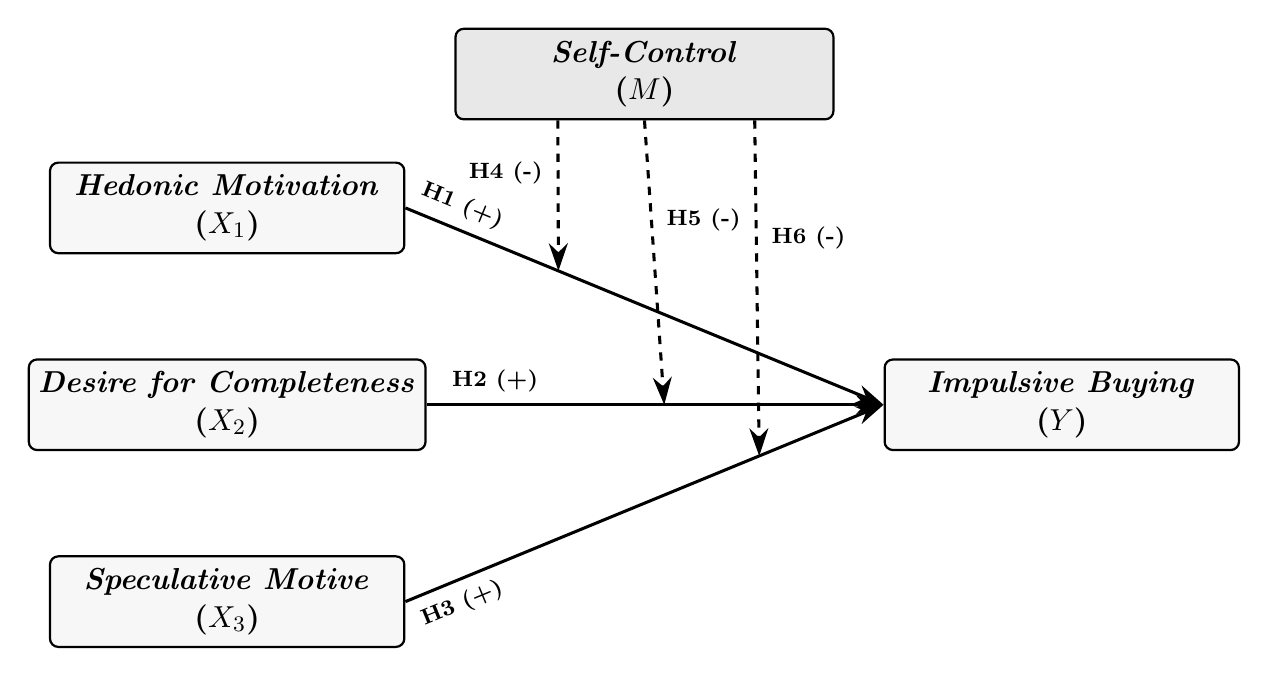
\begin{tikzpicture}[
  box/.style = {
    rectangle, draw=black, thick, fill=gray!6, rounded corners=3pt,
    minimum width=4.5cm, minimum height=1.15cm, align=center,
    font=\fontsize{11}{13.5}\selectfont\bfseries
  },
  modbox/.style = {
    rectangle, draw=black, thick, fill=gray!18, rounded corners=3pt,
    minimum width=4.8cm, minimum height=1.15cm, align=center,
    font=\fontsize{11}{13.5}\selectfont\bfseries
  },
  arrow/.style = {-{Stealth[length=3.5mm, width=2.4mm]}, line width=1.1pt},
  dasharrow/.style = {-{Stealth[length=3.5mm, width=2.4mm]}, line width=1.1pt, dashed}
]

  % Variabel Independen (X) di sebelah kiri (x = 0)
  \node[box] (x1) at (0, 2.5) {\emph{Hedonic Motivation}\\($X_1$)};
  \node[box] (x2) at (0, 0)   {\emph{Desire for Completeness}\\($X_2$)};
  \node[box] (x3) at (0, -2.5){\emph{Speculative Motive}\\($X_3$)};

  % Variabel Dependen (Y) di sebelah kanan (x = 10.6)
  \node[box] (y)  at (10.6, 0) {\emph{Impulsive Buying}\\($Y$)};

  % Variabel Moderasi (M) di atas tengah (x = 5.3, y = 4.2)
  \node[modbox] (m) at (5.3, 4.2) {\emph{Self-Control}\\($M$)};

  % Garis Pengaruh Langsung (H1, H2, H3)
  \draw[arrow] (x1.east) -- (y.west)
    node[pos=0.10, above=2pt, sloped, font=\footnotesize\bfseries, fill=white, inner sep=2pt] {H1 (+)};
  \draw[arrow] (x2.east) -- (y.west)
    node[pos=0.15, above=2pt, font=\footnotesize\bfseries, fill=white, inner sep=2pt] {H2 (+)};
  \draw[arrow] (x3.east) -- (y.west)
    node[pos=0.10, below=2pt, sloped, font=\footnotesize\bfseries, fill=white, inner sep=2pt] {H3 (+)};

  % Titik pertemuan moderasi yang terpisah secara horizontal (Parallel Tracks)
  \coordinate (mod1) at ($(x1.east)!0.32!(y.west)$);
  \coordinate (mod2) at ($(x2.east)!0.52!(y.west)$);
  \coordinate (mod3) at ($(x3.east)!0.74!(y.west)$);

  % Garis Pengaruh Moderasi (H4, H5, H6)
  \draw[dasharrow] ([xshift=-1.1cm]m.south) -- (mod1)
    node[pos=0.35, left=3pt, font=\footnotesize\bfseries, fill=white, inner sep=2pt] {H4 (-)};
  \draw[dasharrow] (m.south) -- (mod2)
    node[pos=0.35, right=3pt, font=\footnotesize\bfseries, fill=white, inner sep=2pt] {H5 (-)};
  \draw[dasharrow] ([xshift=1.4cm]m.south) -- (mod3)
    node[pos=0.35, right=3pt, font=\footnotesize\bfseries, fill=white, inner sep=2pt] {H6 (-)};

\end{tikzpicture}
}
\caption{Model Rerangka Konseptual Penelitian}
\label{fig:rerangka_penelitian}
\begin{flushleft}
  \footnotesize\textit{Keterangan:} Garis lurus menunjukkan pengaruh langsung yang dihipotesiskan (H1, H2, H3); garis putus-putus menunjukkan efek moderasi kontrol diri yang memperlemah (H4, H5, H6). (Catatan: Diagram menampilkan rerangka konseptual hipotesis; dalam model estimasi regresi MRA empiris, efek utama pemoderasi $M$ diikutsertakan sebagai prediktor dasar dalam model aditif baseline. Koefisien $\beta_4$ ($M^* \rightarrow Y$) hanya baseline aditif untuk isolasi $\Delta R^2$, bukan hipotesis tersendiri; tidak ada RM/Tujuan/H untuk efek langsung $M$.)
\end{flushleft}
\end{figure}

% ============================================================
%  BAB 3: METODE PENELITIAN
% ============================================================
\newpage
\setcounter{section}{2}
\section*{BAB 3\\[0.3cm]METODE PENELITIAN}
\addcontentsline{toc}{section}{\texorpdfstring{BAB 3\quad METODE PENELITIAN}{BAB 3 METODE PENELITIAN}}
\setcounter{section}{3}
\setcounter{subsection}{0}
\setcounter{table}{0}
\setcounter{figure}{0}
\setcounter{equation}{0}

\subsection{Jenis dan Sumber Data}

Penelitian ini menguji hipotesis empiris H1--H6 mengenai hubungan struktural antarvariabel dengan pendekatan kuantitatif asosiatif dan desain survei \emph{cross-sectional}. Pendekatan ini dipilih karena kerangka teoritis telah merumuskan hubungan tersebut secara eksplisit. Pengumpulan data primer dilakukan satu kali pada satu titik waktu kepada sampel responden untuk memotret fenomena yang diteliti \citep{sekaran2016research}.

Penulis mengumpulkan data primer langsung dari responden dengan menyebarkan kuesioner daring (\emph{online questionnaire}) melalui Google Forms. Kuesioner tersebut memakai pertanyaan tertutup berskala Likert 5 poin \citep{sugiyono2019metode}, sebagaimana disajikan pada Tabel 3.1:

\begin{table}[H]
\centering
\caption{Skala Pengukuran Likert 5 Poin}
\label{tab:skala_likert}
\begin{tabular}{clc}
\toprule
\textbf{Skor} & \textbf{Pernyataan Sikap} & \textbf{Singkatan} \\
\midrule
1 & Sangat Tidak Setuju & STS \\
2 & Tidak Setuju & TS \\
3 & Netral / Ragu-ragu & N \\
4 & Setuju & S \\
5 & Sangat Setuju & SS \\
\bottomrule
\end{tabular}
\begin{flushleft}
  \footnotesize\textit{Sumber: Dikembangkan dari Sugiyono (2019) untuk instrumen kuesioner penelitian, 2026.}
\end{flushleft}
\end{table}

Data sekunder berasal dari studi kepustakaan. Sumbernya meliputi laporan resmi The Pok\'emon Company dan data agregasi industri hiburan global, dilengkapi buku teks metodologi dan keuangan perilaku serta artikel jurnal nasional dan internasional bereputasi terindeks SINTA dan Scopus.

\subsubsection{Batasan Penelitian dan Ruang Lingkup Operasional}

Penelitian ini menetapkan batasan operasional sebagai berikut:
\begin{enumerate}
  \item \textbf{Batasan Komoditas Objek:} Penelitian ini secara ketat dibatasi pada pembelian produk kemasan acak tertutup (\emph{booster pack}) fisik resmi \emph{Pok\'emon Trading Card Game} (Pok\'emon TCG) berbahasa Indonesia yang dirilis oleh The Pok\'emon Company / AKG Games. Penelitian ini tidak meneliti kartu permainan digital (seperti \emph{Pok\'emon TCG Live} atau \emph{Pok\'emon TCG Pocket}) maupun produk kartu dari waralaba lain (\emph{Yu-Gi-Oh!}, \emph{Magic: The Gathering}, atau \emph{One Piece Card Game}).
  \item \textbf{Batasan Responden:} Subjek penelitian dibatasi pada konsumen dan kolektor Warga Negara Indonesia (WNI) yang berdomisili di Indonesia, berusia minimal 17 tahun, dan memiliki riwayat pembelian aktif \emph{booster pack} fisik minimal 1 kali dalam 12 bulan terakhir (diutamakan 6 bulan terakhir untuk kesegaran recall). Penelitian ini tidak membatasi kohort generasi; penyebutan Generasi Z pada Manfaat Praktis merujuk pada segmen penerima manfaat, bukan pembatas populasi.
  \item \textbf{Batasan Konseptual dan Metodologis:} Variabel yang diteliti dibatasi pada pengaruh tiga variabel independen (\emph{Hedonic Motivation}, \emph{Desire for Completeness}, dan \emph{Speculative Motive}) terhadap satu variabel dependen (\emph{Impulsive Buying}) dengan satu variabel moderasi (\emph{Self-Control}), yang diestimasi menggunakan teknik regresi moderasi (\emph{Moderated Regression Analysis} / MRA) berbantuan perangkat lunak IBM SPSS Statistics.
\end{enumerate}

\subsection{Populasi dan Sampel}

\subsubsection{Populasi dan Identifikasi Sumber Komunitas}

Populasi penelitian ini adalah seluruh konsumen atau kolektor kartu fisik Pok\'emon \emph{Trading Card Game} resmi berbahasa Indonesia di wilayah Republik Indonesia. Populasi ini tergolong tidak terbatas (\emph{infinite / unknown population}) karena jumlah seluruh pembeli kartu tidak dapat diketahui secara pasti mengingat luasnya jaringan distribusi ritel modern di Indonesia.

Keberadaan dan identifikasi populasi sasaran dalam penelitian ini bersumber dari ekosistem nyata komunitas TCG di Indonesia:
\begin{enumerate}
  \item \textbf{Komunitas Toko Hobi Resmi (\emph{Local Game Stores} / LGS):} Jaringan komunitas pemain dan kolektor terdaftar yang aktif berkegiatan di toko hobi resmi mitra AKG Games di wilayah Jabodetabek, Bandung, Surabaya, Yogyakarta, Medan, dan kota-kota besar lainnya.
  \item \textbf{Komunitas Digital Berskala Nasional:} Grup komunitas daring aktif, antara lain grup Facebook \emph{Pok\'emon TCG Indonesia} (dengan puluhan ribu anggota aktif), \emph{server} Discord komunitas pemain kartu Indonesia, serta grup lelang dan jual-beli kartu di WhatsApp dan Telegram.
  \item \textbf{Peserta Turnamen Resmi:} Komunitas pemain yang berpartisipasi dalam ajang kompetisi resmi seperti \emph{Town League} dan \emph{Regional League} yang diselenggarakan secara berkala di Indonesia.
\end{enumerate}

\subsubsection{Sampel dan Justifikasi Kriteria Inklusi}

Penarikan sampel memakai teknik sampel bertujuan (\emph{purposive sampling}). Responden wajib memenuhi kriteria inklusi beserta justifikasi ilmiah berikut:
\begin{enumerate}
  \item \textbf{Warga Negara Indonesia (WNI) dan Berdomisili di Indonesia:} Kriteria ini memastikan responden mengalami langsung dinamika ketersediaan produk kartu resmi berbahasa Indonesia serta struktur harga ritel dan pasar sekunder domestik.
  \item \textbf{Berusia Minimal 17 Tahun pada Saat Pengisian Kuesioner:} 
  \begin{itemize}
    \item \emph{Aspek Kedewasaan Administratif dan Hak Sipil:} Berdasarkan Undang-Undang Republik Indonesia Nomor 24 Tahun 2013 tentang Perubahan atas Undang-Undang Nomor 23 Tahun 2006 tentang Administrasi Kependudukan, batas usia 17 tahun menandai kepemilikan Kartu Tanda Penduduk (KTP) sebagai bukti identitas kedewasaan administratif dan hak sipil di Indonesia. Pada usia ini, responden dipandang cakap memberikan persetujuan partisipasi survei risiko-minimal (\emph{informed consent}) secara sadar dan sukarela. Perlindungan etik: partisipasi sukarela, anonim tanpa nama, data rahasia hanya untuk akademik, responden boleh mundur kapan saja; tanpa memerlukan komite etik formal untuk survei risiko-minimal ini.
    \item \emph{Diskresi Keuangan Mandiri:} Pada usia 17 tahun ke atas (umumnya berada pada jenjang pendidikan akhir SMA atau mahasiswa perguruan tinggi), individu telah memiliki alokasi diskresi keuangan pribadi (uang saku mandiri atau penghasilan kerja paruh waktu) yang dapat dibelanjakan secara independen di gerai kasir minimarket.
    \item \emph{Kapasitas Kognitif:} Memastikan kematangan kognitif responden dalam memahami butir-butir pernyataan kuesioner ilmiah secara objektif dan bertanggung jawab.
  \end{itemize}
  \item \textbf{Pernah Membeli \emph{Booster Pack} Resmi Pok\'emon TCG Fisik Minimal 1 Kali dalam 12 Bulan Terakhir (Diutamakan 6 Bulan Terakhir untuk Kesegaran Recall):}
  \begin{itemize}
    \item \emph{Pengalaman Riil Konsumsi:} Kriteria ini memastikan responden benar-benar pernah mengalami proses pengambilan keputusan belanja di etalase toko dan merasakan sensasi membuka bungkus kartu (\emph{pack opening thrill}).
    \item \emph{Bias Ingatan Retrospektif (\emph{Recall Bias}):} Rentang waktu 12 bulan (diutamakan 6 bulan) lazim dipakai dalam riset perilaku konsumen agar memori kognitif dan luapan afektif saat bertransaksi masih tersimpan segar dalam ingatan responden, sehingga data yang dilaporkan lebih dapat diandalkan.
  \end{itemize}
\end{enumerate}

\subsubsection{Penentuan Ukuran Sampel}

Ukuran sampel minimum yang dipersyaratkan adalah 111 responden, dihitung dengan formula \citet{green1991subjects} untuk analisis regresi linear berganda:
\begin{itemize}
  \item Untuk pengujian model korelasi keseluruhan (\emph{overall model}):
  \begin{equation}
    N \ge 50 + 8k
    \label{eq:sampel_overall}
  \end{equation}
  Dengan $k = 7$ prediktor ($X_1, X_2, X_3, M, X_1 \cdot M, X_2 \cdot M, X_3 \cdot M$), maka:
  \[ N \ge 50 + 8(7) = 50 + 56 = 106\text{ responden} \]
  \item Untuk pengujian prediktor individual (\emph{individual predictors}):
  \begin{equation}
    N \ge 104 + k
    \label{eq:sampel_individual}
  \end{equation}
  \[ N \ge 104 + 7 = 111\text{ responden} \]
\end{itemize}

Hasil perhitungan Green (1991) di atas menetapkan syarat minimum absolut 111 responden. Penelitian ini menargetkan \textbf{120 hingga 150 responden} sebagai sampel bersih yang dapat dianalisis (\emph{usable and analyzable sample}), di luar 30 responden untuk uji coba instrumen (\emph{pilot testing}). Rentang 120--150 tersebut memenuhi kriteria \citet{cohen1988statistical} untuk kekuatan uji (\emph{statistical power}) $\ge 0,80$ pada taraf nyata 5\% dengan asumsi efek sedang (\emph{medium effect size}, $f^2 = 0,15$).

\subsubsection{Justifikasi Komparatif Pemilihan Teknik Sampling}

Literatur metodologi kuantitatif \citep{sekaran2016research, sugiyono2019metode} membagi pengambilan sampel ke dalam dua rumpun utama: \emph{Probability Sampling} dan \emph{Non-Probability Sampling}:
\begin{itemize}
  \item \emph{Probability Sampling} (seperti \emph{Simple Random Sampling} atau \emph{Stratified Random Sampling}) menuntut adanya kerangka sampling (\emph{sampling frame}) yang memuat daftar lengkap seluruh anggota populasi. Kerangka sampling sensus pembeli kartu Pok\'emon di Indonesia tidak tersedia secara terpusat sehingga teknik probabilitas murni tidak dapat diterapkan secara sahih.
  \item Karena itu, penelitian ini memakai rumpun \emph{Non-Probability Sampling} dengan teknik spesifik \textbf{\emph{Purposive Sampling}} (sampel bertujuan) berdasarkan kriteria inklusi yang ditetapkan peneliti.
\end{itemize}

Pemilihan \emph{purposive sampling} merupakan pendekatan yang tepat karena menjamin bahwa data yang dikumpulkan berasal murni dari individu yang memiliki kualifikasi relevan (kolektor/pembeli aktif kartu Pok\'emon resmi berusia dewasa), sehingga data yang diperoleh memiliki kesesuaian dan relevansi sampel yang tinggi terhadap segmen yang diteliti. Temuan bersifat analitis pada segmen WNI berusia minimal 17 tahun pembeli aktif; bukan estimasi probabilistik nasional, karena tanpa \emph{sampling frame} terpusat generalisasi statistik ke seluruh populasi nasional tidak diklaim. Pendekatan \emph{purposive sampling} pada komunitas hobi dan kartu koleksi ini sejalan dengan praktik riset internasional terdahulu pada konteks komunitas kolektor \citep{aryadi2024personal}.

\subsection{Model Penelitian}

Penelitian ini menguji hipotesis dengan prosedur regresi hirarkis \emph{Moderated Regression Analysis} (MRA) berbasis OLS dalam dua model bertahap \citep{aiken1991multiple, cohen1988statistical, hayes2018introduction}. Prosedur ini memisahkan efek moderasi murni dari efek langsung pemoderasi:

\noindent\textbf{Model 1: Regresi Linear Berganda Hirarkis (Model Aditif Baseline / Efek Utama):}
\begin{equation}
  Y = \alpha + \beta_1 X_1^* + \beta_2 X_2^* + \beta_3 X_3^* + \beta_4 M^* + e
  \label{eq:model1_regresi}
\end{equation}

\noindent\textbf{Model 2: \emph{Moderated Regression Analysis} / MRA (Model Interaksi Moderasi Penuh):}
\begin{equation}
  Y = \alpha + \beta_1 X_1^* + \beta_2 X_2^* + \beta_3 X_3^* + \beta_4 M^* + \beta_5 (X_1^* \cdot M^*) + \beta_6 (X_2^* \cdot M^*) + \beta_7 (X_3^* \cdot M^*) + e
  \label{eq:model2_mra}
\end{equation}

\noindent Di mana:
\begin{itemize}[noitemsep,topsep=2pt]
  \item $Y$ = Skor komposit \emph{Impulsive Buying} (variabel dependen)
  \item X1*, X2*, X3* = Skor prediktor terpusat (\emph{mean-centered}), yaitu skor asli dikurangi rata-ratanya, untuk \emph{Hedonic Motivation}, \emph{Desire for Completeness}, dan \emph{Speculative Motive}
  \item M* = Skor \emph{Self-Control} terpusat (\emph{mean-centered}), yaitu skor asli dikurangi rata-ratanya
  \item X1* x M*, X2* x M*, X3* x M* = Istilah interaksi, yaitu perkalian prediktor terpusat dengan pemoderasi terpusat (\emph{interaction terms})
  \item $\alpha$ = Nilai intersep konstan regresi
  \item $\beta_1, \beta_2, \beta_3$ = Koefisien regresi efek utama prediktor pada nilai rata-rata pemoderasi (M* = 0)
  \item $\beta_4$ = Koefisien regresi efek langsung pemoderasi (\emph{Self-Control}) terhadap $Y$
  \item $\beta_5, \beta_6, \beta_7$ = Koefisien regresi interaksi moderasi (H4, H5, H6)
  \item $e$ = \emph{Error term} (residual pengganggu)
\end{itemize}

Penyertaan M* pada Model 1 sebagai garis dasar aditif (\emph{additive baseline}) menjamin bahwa peningkatan koefisien determinasi (selisih R2 Model 2 terhadap R2 Model 1) murni mengisolasi kontribusi penjelas tambahan dari ketiga variabel interaksi moderasi, yang diuji secara simultan melalui statistik $F_{\text{change}}$: Koefisien $\beta_4$ (M* terhadap $Y$) pada Model 1 semata-mata merupakan kontrol baseline aditif agar selisih R2 tidak tercampur efek langsung pemoderasi; $\beta_4$ tidak diuji sebagai hipotesis tersendiri dan tidak memiliki pasangan RM/Tujuan/H (hipotesis penelitian tetap 6: H1--H3 langsung, H4--H6 moderasi memperlemah). Baris 4 pada matriks kesenjangan (Subjek M terhadap $Y$) berfungsi sebagai justifikasi teoretis perlunya memasukkan M* sebagai baseline, bukan sebagai hipotesis tambahan.
\begin{equation}
  F_{\text{change}} = \frac{(R^2_{\text{Model 2}} - R^2_{\text{Model 1}}) / 3}{(1 - R^2_{\text{Model 2}}) / (N - 8)}
  \label{eq:f_change}
\end{equation}
dengan derajat kebebasan $df_1 = 3$ dan $df_2 = N - 8$.

\subsection{Operasionalisasi Variabel}

Operasionalisasi variabel penelitian disajikan secara komprehensif pada Tabel 3.2. Tabel disusun menggunakan format terbuka (\emph{open table}) standar publikasi jurnal tanpa garis vertikal, dengan penataan kolom proporsional:

\begingroup
\singlespacing
\setlength{\tabcolsep}{4pt}
\small
\begin{longtable}{>{\raggedright\arraybackslash}p{2.1cm} >{\raggedright\arraybackslash}p{2.7cm} >{\raggedright\arraybackslash}p{2.0cm} >{\raggedright\arraybackslash}p{4.6cm} >{\centering\arraybackslash}p{1.1cm}}
\caption{Operasionalisasi Variabel Penelitian} \label{tab:operasionalisasi} \\
\toprule
\textbf{Variabel} & \textbf{Definisi Operasional} & \textbf{Dimensi} & \textbf{Indikator Pernyataan} & \textbf{Skala} \\
\midrule
\endfirsthead
\multicolumn{5}{l}{\footnotesize\textit{Lanjutan Tabel \thetable\ -- Operasionalisasi Variabel Penelitian}} \\[0.2cm]
\toprule
\textbf{Variabel} & \textbf{Definisi Operasional} & \textbf{Dimensi} & \textbf{Indikator Pernyataan} & \textbf{Skala} \\
\midrule
\endhead
\midrule
\multicolumn{5}{r}{\footnotesize\textit{Bersambung ke halaman berikutnya}} \\
\endfoot
\bottomrule
\endlastfoot

\textbf{\emph{Impulsive Buying} ($Y$)} & Kecenderungan membeli \emph{booster pack} Pok\'emon TCG tanpa rencana awal dan didorong emosi sesaat \citep{rook1987buying, verplanken2001individual}. & Kognitif & Y1. Saya sering membeli \emph{booster pack} kartu Pok\'emon tanpa rencana anggaran sebelumnya. & Likert 1--5 \\
\addlinespace[3pt]
& & Kognitif & Y2. Saya tidak mempertimbangkan dampak finansial saat membeli kartu Pok\'emon di toko. & Likert 1--5 \\
\addlinespace[3pt]
& & Afektif & Y3. Saya merasa terdorong secara spontan untuk membeli \emph{pack} saat melihatnya di etalase toko. & Likert 1--5 \\
\addlinespace[3pt]
& & Afektif & Y4. Saya merasakan kegembiraan sesaat ketika memutuskan membeli kartu secara mendadak. & Likert 1--5 \\
\addlinespace[3pt]
& & Kognitif & Y5. Saya sering membeli \emph{pack} lebih banyak dari yang semula saya niatkan. & Likert 1--5 \\
\addlinespace[3pt]
& & Afektif & Y6. Saya sulit menahan hasrat berbelanja kartu Pok\'emon saat rilis seri baru. & Likert 1--5 \\
\midrule
\textbf{\emph{Hedonic Motivation} ($X_1$)} & Motivasi belanja untuk kesenangan emosional dan sensasi petualangan \citep{arnold2003hedonic}. & \emph{Adventure} & X1.1. Membuka kemasan \emph{booster pack} memberikan sensasi petualangan dan kejutan mendebarkan. & Likert 1--5 \\
\addlinespace[3pt]
& & \emph{Gratification} & X1.2. Membeli kartu Pok\'emon adalah cara saya menghibur diri dan meredakan stres. & Likert 1--5 \\
\addlinespace[3pt]
& & \emph{Social} & X1.3. Berbelanja kartu Pok\'emon mempererat ikatan dan kebersamaan dengan sesama teman sehobi. & Likert 1--5 \\
\addlinespace[3pt]
& & \emph{Role} & X1.4. Saya menikmati berbelanja kartu Pok\'emon untuk dihadiahkan atau dimainkan bersama teman dan keluarga sehobi. & Likert 1--5 \\
\addlinespace[3pt]
& & \emph{Idea} & X1.5. Saya senang mengikuti tren rilis seri kartu Pok\'emon dan inovasi desain terbarunya. & Likert 1--5 \\
\midrule
\textbf{\emph{Desire for Completeness} ($X_2$)} & Dorongan psikologis menuntaskan set koleksi akibat \emph{Zeigarnik Effect} \citep{belk1995collecting, gao2014completing, barasz2017pseudo}. & \emph{Cognitive Tension} & X2.1. Saya merasa tidak nyaman ketika album koleksi kartu Pok\'emon saya memiliki slot kosong. & Likert 1--5 \\
\addlinespace[3pt]
& & \emph{Drive for Closure} & X2.2. Hasrat melengkapi seluruh seri kartu dalam binder mendorong saya untuk terus menambah koleksi. & Likert 1--5 \\
\addlinespace[3pt]
& & \emph{Cognitive Tension} & X2.3. Mengetahui ada kartu yang belum saya miliki dalam suatu seri membuat saya ingin segera membelinya. & Likert 1--5 \\
\addlinespace[3pt]
& & \emph{Wholeness} & X2.4. Melengkapi satu set penuh kartu Pok\'emon memberikan perasaan pencapaian dan kepuasan batin. & Likert 1--5 \\
\addlinespace[3pt]
& & \emph{Drive for Closure} & X2.5. Semakin sedikit kartu yang kurang dalam satu seri, semakin kuat desakan psikologis saya untuk menuntaskannya. & Likert 1--5 \\
\midrule
\textbf{\emph{Speculative Motive} ($X_3$)} & Ekspektasi memperoleh keuntungan finansial dari apresiasi harga di pasar sekunder \citep{shiller2000irrational, baur2018bitcoin, colline2024biases}. & Apresiasi Modal & X3.1. Saya membeli kartu dengan ekspektasi menarik kartu langka bernilai jual tinggi. & Likert 1--5 \\
\addlinespace[3pt]
& & Likuiditas & X3.2. Saya yakin kartu Pok\'emon langka memiliki likuiditas tinggi sehingga mudah dan cepat dijual kembali menjadi uang tunai di pasar sekunder. & Likert 1--5 \\
\addlinespace[3pt]
& & Tren Nilai & X3.3. Saya memandang kartu Pok\'emon langka sebagai aset alternatif yang nilainya dapat naik di masa depan. & Likert 1--5 \\
\addlinespace[3pt]
& & Potensi Nilai & X3.4. Saya memandang biaya pembelian kartu sebanding dengan potensi apresiasi keuntungan di pasar sekunder. & Likert 1--5 \\
\addlinespace[3pt]
& & \emph{Grading Value} & X3.5. Saya tertarik dengan sertifikasi kondisi fisik dan keaslian (\emph{grading}) kartu demi menaikkan nilai jual lelang di pasar sekunder. & Likert 1--5 \\
\midrule
\textbf{\emph{Self-Control} ($M$)} & Kapasitas volisional menolak godaan belanja spontan dan menunda kepuasan sesaat \citep{tangney2004high, vohs2007spent, sultan2012building, apidana2022peran, lienardy2026role}. & Tahan Godaan & M1. Saya mampu menolak godaan berbelanja jika barang tersebut berada di luar rencana anggaran saya. & Likert 1--5 \\
\addlinespace[3pt]
& & Non-Impulsif & M2. Saya terbiasa berpikir tenang dan mempertimbangkan konsekuensi keuangan sebelum memutuskan bertransaksi. & Likert 1--5 \\
\addlinespace[3pt]
& & Tunda Kepuasan & M3. Saya mampu menahan diri dari kesenangan belanja saat ini demi menjaga stabilitas keuangan masa depan. & Likert 1--5 \\
\addlinespace[3pt]
& & Disiplin Diri & M4. Saya memiliki pengendalian diri yang kokoh untuk menahan dorongan membeli barang secara spontan saat melihat barang menarik. & Likert 1--5 \\
\addlinespace[3pt]
& & Kontrol Emosi & M5. Saya tidak mudah terhanyut oleh emosi sesaat dalam membelanjakan uang pribadi. & Likert 1--5 \\
\addlinespace[3pt]
& & Taat Anggaran & M6. Saya secara konsisten mematuhi alokasi batas anggaran pengeluaran hobi yang telah saya tetapkan. & Likert 1--5 \\
\end{longtable}
\endgroup

\subsection{Metode Analisis Data}

\subsubsection{Justifikasi Komparatif Pemilihan Metode Analisis}

Dalam pengujian model penelitian kuantitatif eksplanatori yang melibatkan efek moderasi, terdapat beberapa alternatif metode analisis dalam literatur statistik:
\begin{enumerate}
  \item \textbf{\emph{Structural Equation Modeling} (SEM) Berbasis Kovarians (SEM-CB) atau Varian (SEM-PLS):} Cocok untuk model bertingkat dengan konstruk laten kompleks dan variabel mediasi simultan. Namun, SEM-CB menuntut asumsi distribusi normal multivariat yang sangat ketat serta sampel besar ($N > 200$), sedangkan SEM-PLS lebih ditujukan untuk pemodelan prediktif eksploratif \citep{hair2019multivariate}.
  \item \textbf{\emph{Moderated Regression Analysis} (MRA) Berbasis \emph{Ordinary Least Squares} (OLS):} Merupakan metode klasik dan baku yang dirancang khusus untuk menguji apakah kekuatan atau arah hubungan antara variabel independen dan dependen dipengaruhi oleh variabel pemoderasi kuantitatif \citep{aiken1991multiple, hayes2018introduction, ghozali2018aplikasi}.
\end{enumerate}

Penelitian ini menetapkan \textbf{MRA berbasis OLS berbantuan IBM SPSS Statistics} sebagai metode yang dipilih, dengan pertimbangan metodologis sebagai berikut:
\begin{itemize}
  \item Seluruh variabel penelitian diukur menggunakan skala komposit teruji dengan indikator-indikator yang terdefinisi secara terfokus.
  \item Ukuran sampel penelitian (120--150 responden) berada pada rentang yang sangat ideal dan kokoh untuk OLS, tanpa menimbulkan risiko estimasi berlebih (\emph{over-parameterization}) yang sering terjadi pada SEM \citep{hair2019multivariate}.
  \item Prosedur pemusatan nilai rata-rata (\emph{mean-centering}) diterapkan pada prediktor dan pemoderasi (skor asli dikurangi rata-ratanya), yang secara efektif mereduksi multikolinearitas non-esensial antara variabel prediktor dengan produk interaksinya tanpa mengubah nilai prediksi model ($R^2$) maupun koefisien interaksi, serta memfasilitasi interpretasi koefisien efek utama $\beta_1, \beta_2, \beta_3$ pada nilai rata-rata pemoderasi ($M^* = 0$) \citep{aiken1991multiple, hayes2018introduction}.
  \item Metode ini telah dipakai sejumlah penelitian untuk menguji moderasi kontrol diri terhadap perilaku pembelian impulsif \citep{sultan2012building, apidana2022peran, lienardy2026role}.
\end{itemize}

Tahapan analisis data dilaksanakan sebagai berikut:
\begin{enumerate}
  \item \textbf{Tahap 1: Penyusunan Skor Komposit dan Uji Kualitas Data.} Skor tiap variabel merupakan nilai rata-rata (\emph{mean composite}) dari seluruh butir indikator yang valid pada variabel tersebut. Seluruh butir dikodekan searah dan positif (skor 5 menunjukkan tingkatan konstruk tertinggi). Instrumen diuji kualitasnya sebelum estimasi regresi melalui: (a) \textbf{Uji Validitas Butir} dengan teknik korelasi butir-total Pearson (\emph{Pearson product-moment item-total}) terhadap skor komposit konstruk tujuan. Koefisien korelasi Pearson berkisar -1 hingga +1 (angka 1--5 merupakan rentang skala Likert butir, bukan rentang korelasi). Butir dinyatakan valid jika $r_{\text{hitung}} > r_{\text{tabel}}$ pada taraf nyata 5\% dua sisi ($df=n-2$; pilot $n=30$, yakni $r_{\text{tabel}}$ sekitar 0,361), dengan korelasi \emph{corrected item-total} $\ge 0{,}30$ sebagai pendukung; (b) \textbf{Uji Reliabilitas Konsistensi Internal} dengan koefisien \emph{Cronbach's Alpha}. Konstruk dinyatakan reliabel jika \emph{Cronbach's Alpha} $\ge 0,70$ \citep{ghozali2018aplikasi, sekaran2016research}.

  \item \textbf{Tahap 2: Uji Asumsi Klasik.} Untuk memastikan prasyarat estimasi regresi OLS agar parameter penduga tidak bias dan konsisten: (a) \textbf{Uji Normalitas Residual} dengan \emph{One-Sample Kolmogorov-Smirnov} (residual normal jika signifikansi asimtotik $p > 0,05$); (b) \textbf{Uji Multikolinearitas} melalui \emph{Tolerance} ($> 0,10$) dan \emph{Variance Inflation Factor} (VIF $< 10$) pada Model 1/efek utama (VIF tinggi pada blok interaksi Model 2 pasca-\emph{mean-centering} yang didorong teori tidak serta-merta dinyatakan pelanggaran, karena korelasi struktural prediktor--interaksi bersifat ekspektasian dan \emph{centering} hanya mereduksi multikolinearitas non-esensial); (c) \textbf{Uji Heteroskedastisitas} dengan uji Glejser (model bebas heteroskedastisitas apabila signifikansi parameter terhadap nilai absolut residual $p > 0,05$).
\emph{Catatan metodologis:} Uji autokorelasi (seperti uji Durbin-Watson) sengaja tidak dilakukan karena pengujian autokorelasi secara teoritis hanya relevan untuk data runtun waktu (\emph{time-series}) atau data panel berurutan, bukan untuk survei \emph{cross-sectional} primer \citep{ghozali2018aplikasi}.

  \item \textbf{Tahap 3: Estimasi Regresi Hirarkis dan MRA.} Analisis regresi dilakukan dalam dua tahapan hirarkis berurutan: (a) \textbf{Model 1 Aditif Baseline (Persamaan 3.3):} mengestimasi efek utama ketiga variabel anteseden terpusat ($X_1^*, X_2^*, X_3^*$) beserta efek langsung variabel pemoderasi terpusat ($M^*$) terhadap $Y$; (b) \textbf{Model 2 Interaksi Penuh MRA (Persamaan 3.4):} memasukkan blok tiga istilah interaksi terpusat ($X_1^* \cdot M^*, X_2^* \cdot M^*, X_3^* \cdot M^*$) untuk menguji efek moderasi kontrol diri secara simultan dan parsial.

  \item \textbf{Tahap 4: Uji Koefisien Determinasi ($R^2$) dan Uji F Perubahan.} Kecocokan model dinilai dari \emph{Adjusted} $R^2$ pada Model 1 dan Model 2 sebagai deskriptif. Kontribusi murni blok moderasi terlihat pada peningkatan $R^2$ biasa ($\Delta R^2 = R^2_{\text{Model 2}} - R^2_{\text{Model 1}}$, bukan dari \emph{Adjusted} $R^2$), yang diuji dengan $F_{\text{change}}$ pada taraf nyata 5\% ($p < 0{,}05$) (Persamaan 3.5).

  \item \textbf{Tahap 5: Uji Hipotesis dan Analisis Kemiringan Bersyarat (\emph{Simple Slopes}).} (a) \textbf{Uji Statistik t (Uji Parsial):} menguji signifikansi masing-masing koefisien regresi secara individual pada taraf nyata 5\% (uji dua sisi yang konservatif; hipotesis satu arah H1--H6 dinyatakan didukung jika nilai signifikansi dua sisi $p < 0,05$ dan arah koefisien sejalan dengan arah hipotesis: $\beta_1, \beta_2, \beta_3 > 0$; $\beta_5, \beta_6, \beta_7 < 0$). Koefisien $\beta_1, \beta_2, \beta_3$ pada Model 2 merefleksikan pengaruh utama pada rata-rata kontrol diri ($M^* = 0$); (b) \textbf{Uji Statistik F (Uji Kelayakan Model):} menguji kelayakan model regresi secara simultan pada taraf signifikansi $p < 0,05$; (c) \textbf{Analisis Kemiringan Bersyarat (\emph{Simple Slopes Analysis}):} Hipotesis moderasi (H4, H5, H6) diuji lewat kemiringan bersyarat per-hipotesis; H4: $\frac{\partial Y}{\partial X_1^*} = \beta_1 + \beta_5 M^*$; H5: $\frac{\partial Y}{\partial X_2^*} = \beta_2 + \beta_6 M^*$; H6: $\frac{\partial Y}{\partial X_3^*} = \beta_3 + \beta_7 M^*$ - pada kontrol diri rendah ($-1\,\text{SD}$), rata-rata ($0\,\text{SD}$), dan tinggi ($+1\,\text{SD}$). Efek memperlemah terbukti bila kemiringan $X_i$ terhadap $Y$ mendatar pada kontrol diri tinggi \citep{aiken1991multiple, hayes2018introduction}.
\end{enumerate}

\subsection{Diagram Alur Penelitian}

Tahapan pelaksanaan penelitian ini dari awal perumusan gagasan hingga penarikan kesimpulan disajikan secara skematis pada Gambar 3.1:

\begin{figure}[H]
\centering
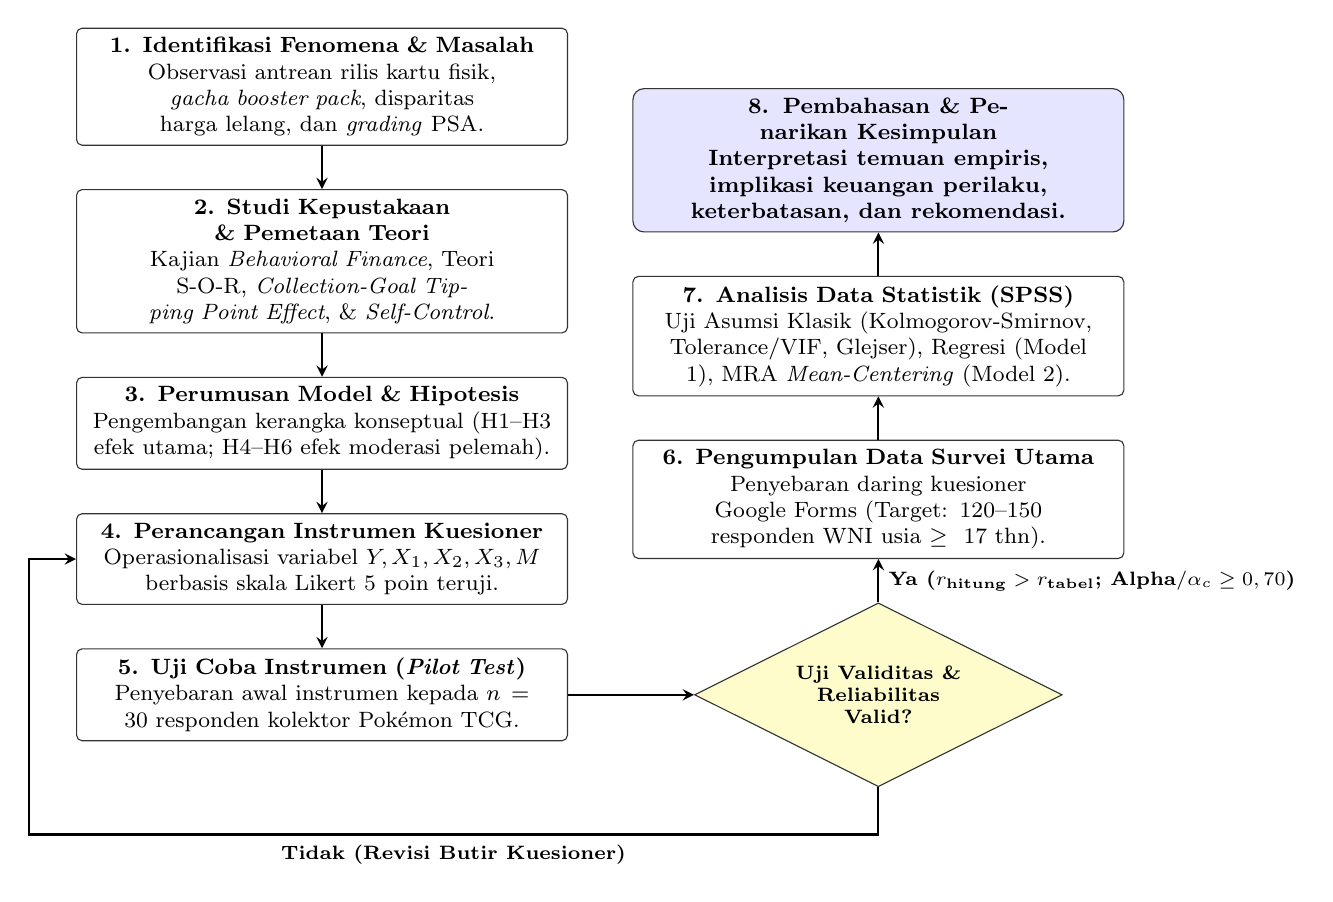
\begin{tikzpicture}[
  node distance=0.55cm and 1.6cm,
  auto,
  startstop/.style={rectangle, rounded corners=4pt, minimum width=6.2cm, minimum height=0.85cm, align=center, text width=6.0cm, draw=black!80, fill=blue!10, font=\footnotesize\bfseries},
  process/.style={rectangle, rounded corners=2pt, minimum width=6.2cm, minimum height=0.85cm, align=center, text width=6.0cm, draw=black!80, fill=white, font=\footnotesize},
  decision/.style={diamond, aspect=2, minimum width=3.0cm, minimum height=1.1cm, align=center, text width=2.5cm, draw=black!80, fill=yellow!20, font=\scriptsize\bfseries},
  arrow/.style={thick, ->, >=stealth}
]

  % Kolom Kiri: Tahap Persiapan & Pengembangan
  \node (step1) [process] {\textbf{1. Identifikasi Fenomena \& Masalah}\\Observasi antrean rilis kartu fisik, \emph{gacha booster pack}, disparitas harga lelang, dan \emph{grading} PSA.};
  \node (step2) [process, below=of step1] {\textbf{2. Studi Kepustakaan \& Pemetaan Teori}\\Kajian \emph{Behavioral Finance}, Teori S-O-R, \emph{Collection-Goal Tipping Point Effect}, \& \emph{Self-Control}.};
  \node (step3) [process, below=of step2] {\textbf{3. Perumusan Model \& Hipotesis}\\Pengembangan kerangka konseptual (H1--H3 efek utama; H4--H6 efek moderasi pelemah).};
  \node (step4) [process, below=of step3] {\textbf{4. Perancangan Instrumen Kuesioner}\\Operasionalisasi variabel $Y, X_1, X_2, X_3, M$ berbasis skala Likert 5 poin teruji.};
  \node (step5) [process, below=of step4] {\textbf{5. Uji Coba Instrumen (\emph{Pilot Test})}\\Penyebaran awal instrumen kepada $n = 30$ responden kolektor Pok\'emon TCG.};

  % Kolom Kanan: Tahap Pengujian & Analisis
  \node (step6) [decision, right=1.6cm of step5] {Uji Validitas \&\\Reliabilitas Valid?};
  \node (step7) [process, above=of step6] {\textbf{6. Pengumpulan Data Survei Utama}\\Penyebaran daring kuesioner Google Forms (Target: 120--150 responden WNI usia $\ge 17$ thn).};
  \node (step8) [process, above=of step7] {\textbf{7. Analisis Data Statistik (SPSS)}\\Uji Asumsi Klasik (Kolmogorov-Smirnov, Tolerance/VIF, Glejser), Regresi (Model 1), MRA \emph{Mean-Centering} (Model 2).};
  \node (step9) [startstop, above=of step8] {\textbf{8. Pembahasan \& Penarikan Kesimpulan}\\Interpretasi temuan empiris, implikasi keuangan perilaku, keterbatasan, dan rekomendasi.};

  % Garis Alur
  \draw [arrow] (step1) -- (step2);
  \draw [arrow] (step2) -- (step3);
  \draw [arrow] (step3) -- (step4);
  \draw [arrow] (step4) -- (step5);
  \draw [arrow] (step5) -- (step6);
  \draw [arrow] (step6) -- node [midway, right, font=\scriptsize\bfseries] {Ya ($r_{\text{hitung}} > r_{\text{tabel}}$; $\text{Alpha}/\alpha_c \ge 0,70$)} (step7);
  \draw [arrow] (step6.south) -- ++(0,-0.6) -| node [pos=0.25, below, font=\scriptsize\bfseries] {Tidak (Revisi Butir Kuesioner)} ([xshift=-0.6cm]step4.west) |- (step4.west);
  \draw [arrow] (step7) -- (step8);
  \draw [arrow] (step8) -- (step9);

\end{tikzpicture}
\caption{Diagram Alur Pelaksanaan Penelitian}
\label{fig:alur_penelitian}
\begin{flushleft}
  \footnotesize\textit{Sumber: Dikembangkan oleh penulis untuk tahapan operasional penelitian, 2026.}
\end{flushleft}
\end{figure}

\noindent Masukan dan keluaran tiap tahap pada Gambar 3.1 adalah sebagai berikut:
\begin{enumerate}[noitemsep,topsep=2pt]
  \item \textbf{Tahap 1:} Masukan berupa observasi antrean rilis dan disparitas harga; keluaran berupa rumusan fenomena dan masalah penelitian.
  \item \textbf{Tahap 2:} Masukan berupa fenomena teridentifikasi; keluaran berupa peta teori dan anteseden terpilih ($X_1, X_2, X_3, M$).
  \item \textbf{Tahap 3:} Masukan berupa peta teori; keluaran berupa kerangka konseptual dan hipotesis H1--H6.
  \item \textbf{Tahap 4:} Masukan berupa kerangka konseptual; keluaran berupa kuesioner operasional (Tabel 3.1 dan 3.2).
  \item \textbf{Tahap 5:} Masukan berupa kuesioner draf; keluaran berupa data percontohan $n=30$ beserta evaluasi butir.
  \item \textbf{Keputusan validitas:} Masukan berupa data percontohan; keluaran berupa keputusan lanjut (instrumen valid dan reliabel) atau revisi butir.
  \item \textbf{Tahap 6:} Masukan berupa instrumen final; keluaran berupa data survei utama $n=120$--$150$.
  \item \textbf{Tahap 7:} Masukan berupa data survei utama; keluaran berupa hasil uji asumsi klasik (Kolmogorov-Smirnov, Tolerance/VIF, Glejser), estimasi Model 1--Model 2, nilai $\Delta R^2$ dan $F_{\text{change}}$, serta uji H1--H6.
  \item \textbf{Tahap 8:} Masukan berupa seluruh hasil analisis; keluaran berupa pembahasan, kesimpulan, keterbatasan, dan rekomendasi.
\end{enumerate}

\subsection{Jadwal Pelaksanaan Penelitian}

Jadwal pelaksanaan tahapan kegiatan penelitian direncanakan berlangsung selama 6 (enam) bulan kalender, sebagaimana dirangkum pada Tabel 3.3:

\begin{table}[H]
\centering
\caption{Jadwal Pelaksanaan Kegiatan Penelitian (Tahun 2026)}
\label{tab:jadwal_penelitian}
\begin{tabularx}{\textwidth}{c X cccccc}
\toprule
\multirow{2}{*}{\textbf{No}} & \multirow{2}{*}{\textbf{Tahapan Kegiatan Penelitian}} & \multicolumn{6}{c}{\textbf{Bulan Pelaksanaan}} \\
\cmidrule(lr){3-8}
& & \textbf{B1} & \textbf{B2} & \textbf{B3} & \textbf{B4} & \textbf{B5} & \textbf{B6} \\
\midrule
1 & Identifikasi fenomena pasar dan perumusan topik & $\bullet$ & & & & & \\
2 & Studi kepustakaan dan telaah literatur jurnal & $\bullet$ & $\bullet$ & & & & \\
3 & Penyusunan naskah proposal penelitian (Bab 1--3) & & $\bullet$ & $\bullet$ & & & \\
4 & Bimbingan intensif dan revisi proposal skripsi & & $\bullet$ & $\bullet$ & & & \\
5 & Pelaksanaan Seminar Proposal Skripsi & & & $\bullet$ & & & \\
6 & Uji coba instrumen kuesioner (\emph{pilot test} $n=30$) & & & & $\bullet$ & & \\
7 & Pengumpulan data lapangan survei utama ($n=120$--$150$) & & & & $\bullet$ & $\bullet$ & \\
8 & Tabulasi data dan pengolahan statistik via SPSS & & & & & $\bullet$ & \\
9 & Penyusunan laporan Bab 4 (Analisis) dan Bab 5 (Penutup) & & & & & $\bullet$ & $\bullet$ \\
10 & Ujian Sidang Skripsi dan Komprehensif & & & & & & $\bullet$ \\
\bottomrule
\end{tabularx}
\begin{flushleft}
  \footnotesize\textit{Keterangan: B1 = Bulan ke-1; B2 = Bulan ke-2; B3 = Bulan ke-3; B4 = Bulan ke-4; B5 = Bulan ke-5; B6 = Bulan ke-6 tahun akademik 2026.}
\end{flushleft}
\end{table}

% ============================================================
%  DAFTAR PUSTAKA
% ============================================================
\newpage
\renewcommand{\refname}{DAFTAR PUSTAKA}
\addcontentsline{toc}{section}{DAFTAR PUSTAKA}
\bibliography{references}

\end{document}
